\chapter[Application of models to HSI data]{Application of analytical tissue models to Hyperspectral Imaging data}\label{chap:HSImodel}
\begin{center}
\begin{minipage}[b]{0.9\linewidth}
\small
\textbf{Foreword\,}
This chapter is as yet unpublished. 
\newline
AB has conducted all of the research presented in this chapter under the supervision of JS, MB, and TV. The gelatin-based phantom images were kindly annotated by OM with the NHSI datasets being obtained via a collaborative study between KCL and HVS. 
\end{minipage}
\end{center}

\section{Introduction}
As described in Chapter \ref{chap:intro}, hyperspectral imaging (HSI) is able to capture spatially resolved, diffuse reflectance spectra via non-contact imaging\cite{Lu2014,Giannoni2018,Calin2014,Shapey2019}. It has been posed that this could enable quantitative, spatially-resolved, tissue oxygenation ($StO_2$) extraction from intra-operative HSI data, with the analytical models investigated in Chapters \ref{chap:1layer} and \ref{chap:2layer} being some of the prominent methods of doing so \cite{Yudovsky2009, Jacques1999, Clancy2015, Clancy2020}. 

HSI data is often of lower spectral resolution than the spectrophotometer data tested in the previous chapters, particularly that of snapshot HSI data which compromises spectral resolution in favour of shorter aquisition times\cite{Geelen2014}. Additionally, Hyperspectral imaging is known to suffer from spectral noise which may be reduced significantly by spatial averaging until comparable to traditional optical methods \cite{Zhang2020}.

In this chapter, I will quantify the impact of reducing the spectral resolution and introduction of noise on the performance of the analytical models investigated in Chapters \ref{chap:1layer} and \ref{chap:2layer} by simulating a snapshot camera response from the Monte Carlo datasets used in these previous chapters. These impacts are then evaluated with experimental HSI data of the phantoms detailed in Chapter \ref{chap:1layer}. Finally, the models are applied to a subset of neurosurgical HSI data obtained intra-operatively as part of the HELICoiD and NHSI datasets. 

\section{Methods}
\subsection{Camera response simulation from Monte Carlo datasets}\label{sec:MCcameras}
To obtain datasets of simulated data with known ground truth parameters, the datasets described in Sections \ref{sec:methodsMC} and \ref{sec:methodreference2} are used. For each spectrum in the dataset, the camera response is simulated by convolving the band responses of the snapshot HSI camera (depicted in Figure \ref{fig:rulerspectrum}) and the integral of this is divided by the band response integral as defined in Equation \ref{eq:simulatingcam}. 
\begin{equation}
	c_{n} = \frac{\int r(\lambda)b_n(\lambda) d\lambda}{\int b_n(\lambda) d\lambda}
\label{eq:simulatingcam}
\end{equation}
Here $c_n$ is the measured value from band $n$ by the camera when the true spectrum is $r(\lambda)$ and the band response for this band is $b_n(\lambda)$. Random Gaussian noise can also be added at this stage where the mean is taken to be 0 and varying standard deviations ($\sigma$) are added. $c_n$ is then corrected using an correction matrix to account for the parasitic cross-talk effects as in \ref{methodnecessity}. An example of the stages of this process can be seen in Figure \ref{fig:simulatingcam}. This allows a variety of datasets to be simulated with the same set of ground truth parameters for both quantitative and mean-normalised relative data. Two noise levels are investigated alongside noiseless simulations where the maximum noise level ($\sigma = 0.03$ before mean normalisation) is similar to the standard deviation size seen in the highly controlled dataset investigated in Chapter \ref{chap:SWB}.  
\begin{figure}[h!]
    \centering 
    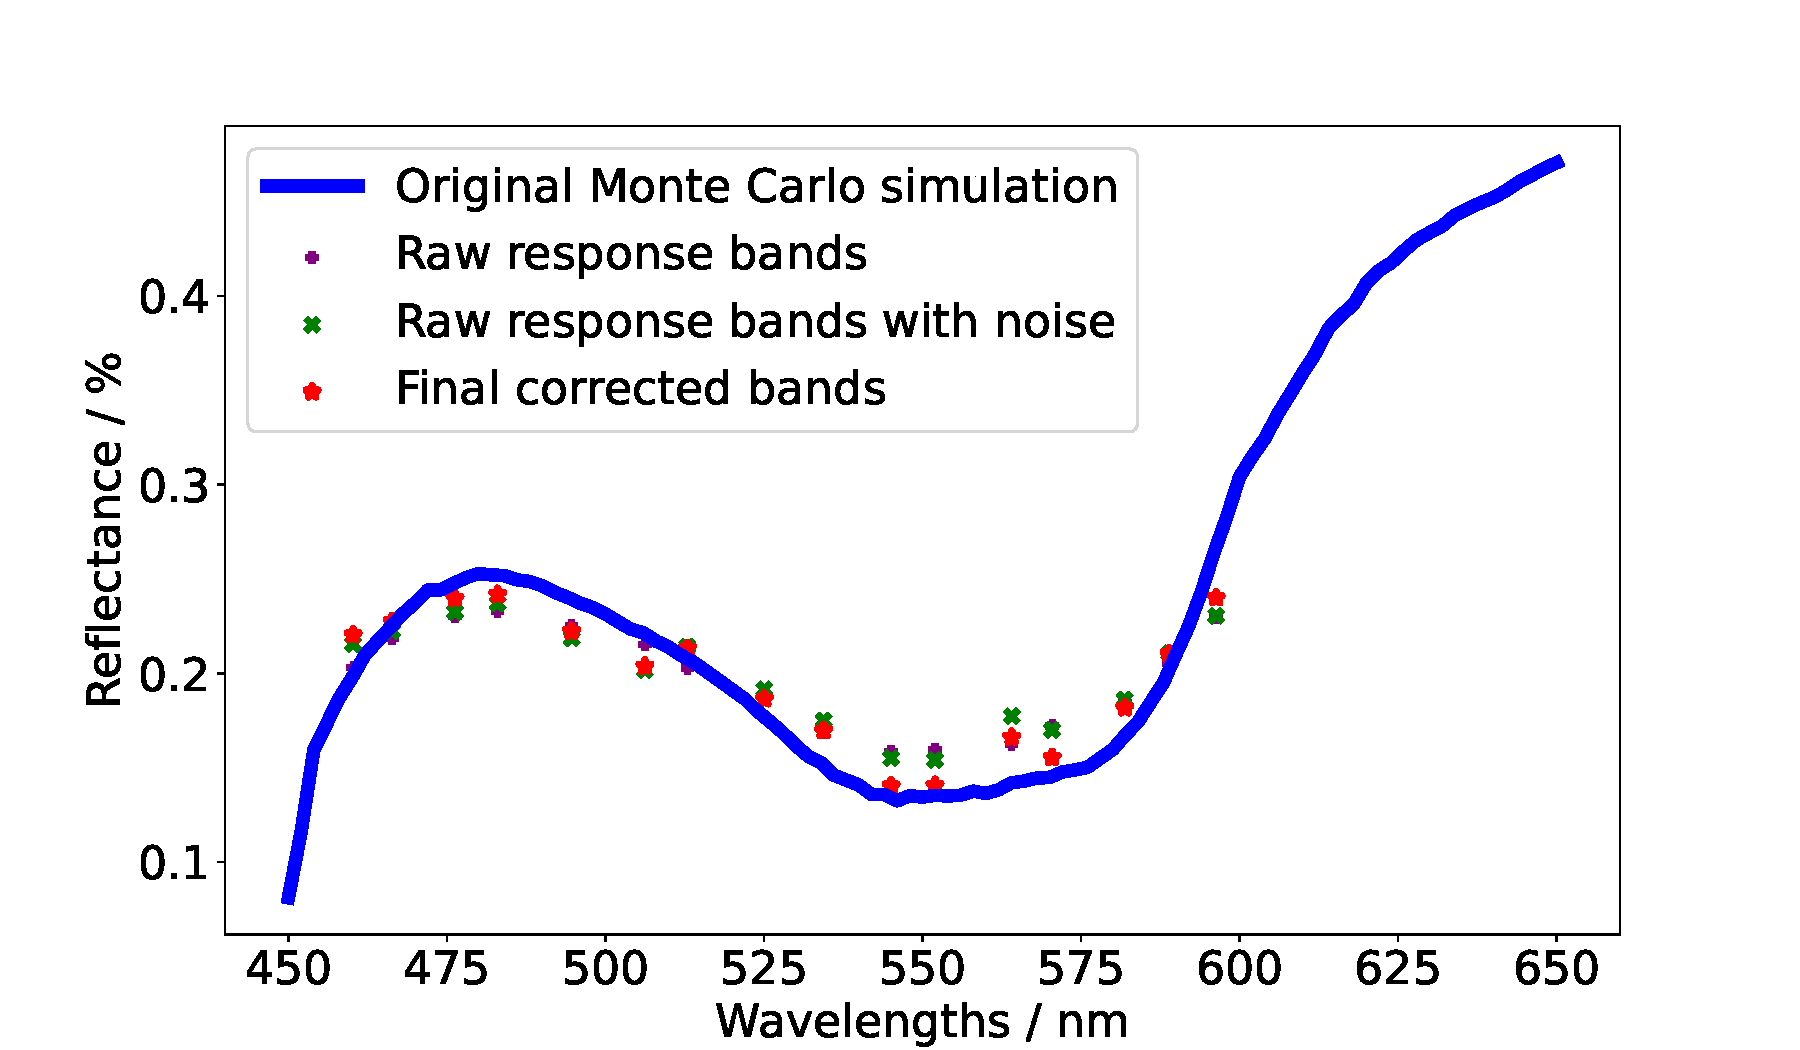
\includegraphics[width=0.7\textwidth]{simulatingcam.pdf}
    \caption{An example of the stages of converting a Monte Carlo diffuse reflectance spectrum (\textcolor{blue}{blue solid}) to a simulated camera response (\textcolor{red}{red $*$}) via the band response convolution (\textcolor{purple}{purple $+$}), the noise addition (\textcolor{MyGreen}{green $\times$}), and finally cross-talk correction.}
    \label{fig:simulatingcam}
\end{figure}

\subsection{Hyperspectral imaging of gelatin-based phantoms}\label{sec:imagingphantoms}
To obtain a measured hyperspectral dataset with known ground truth, HSI images are taken of the two-dye configuration gelatin-based phantoms detailed in Section \ref{sec:methodsphantoms}. The imaging configuration is similar to that described in Section \ref{materials} using a 4x4 16 band visible range snapshot mosaic camera (Ximea utilising the IMEC CMV2K-SSM4X4-VIS sensor, Germany) alongside an f=35mm coupler (Karl Storz, NDTec, VCam HD-F-35 - Camera Lens Adapter, Germany), a $0^\circ$ exoscope (Karl Storz Endoscopy, VITOM Telescope 0° w Integ. Illuminator, UK) and a Xenon light source (Karl Storz Endoscopy, Cold Light Fountain D light C, UK), as detailed in \cite{Ebner2021} and pictured in Figure \ref{fig:imagephantoms}.
\begin{figure}[h!]
    \centering
    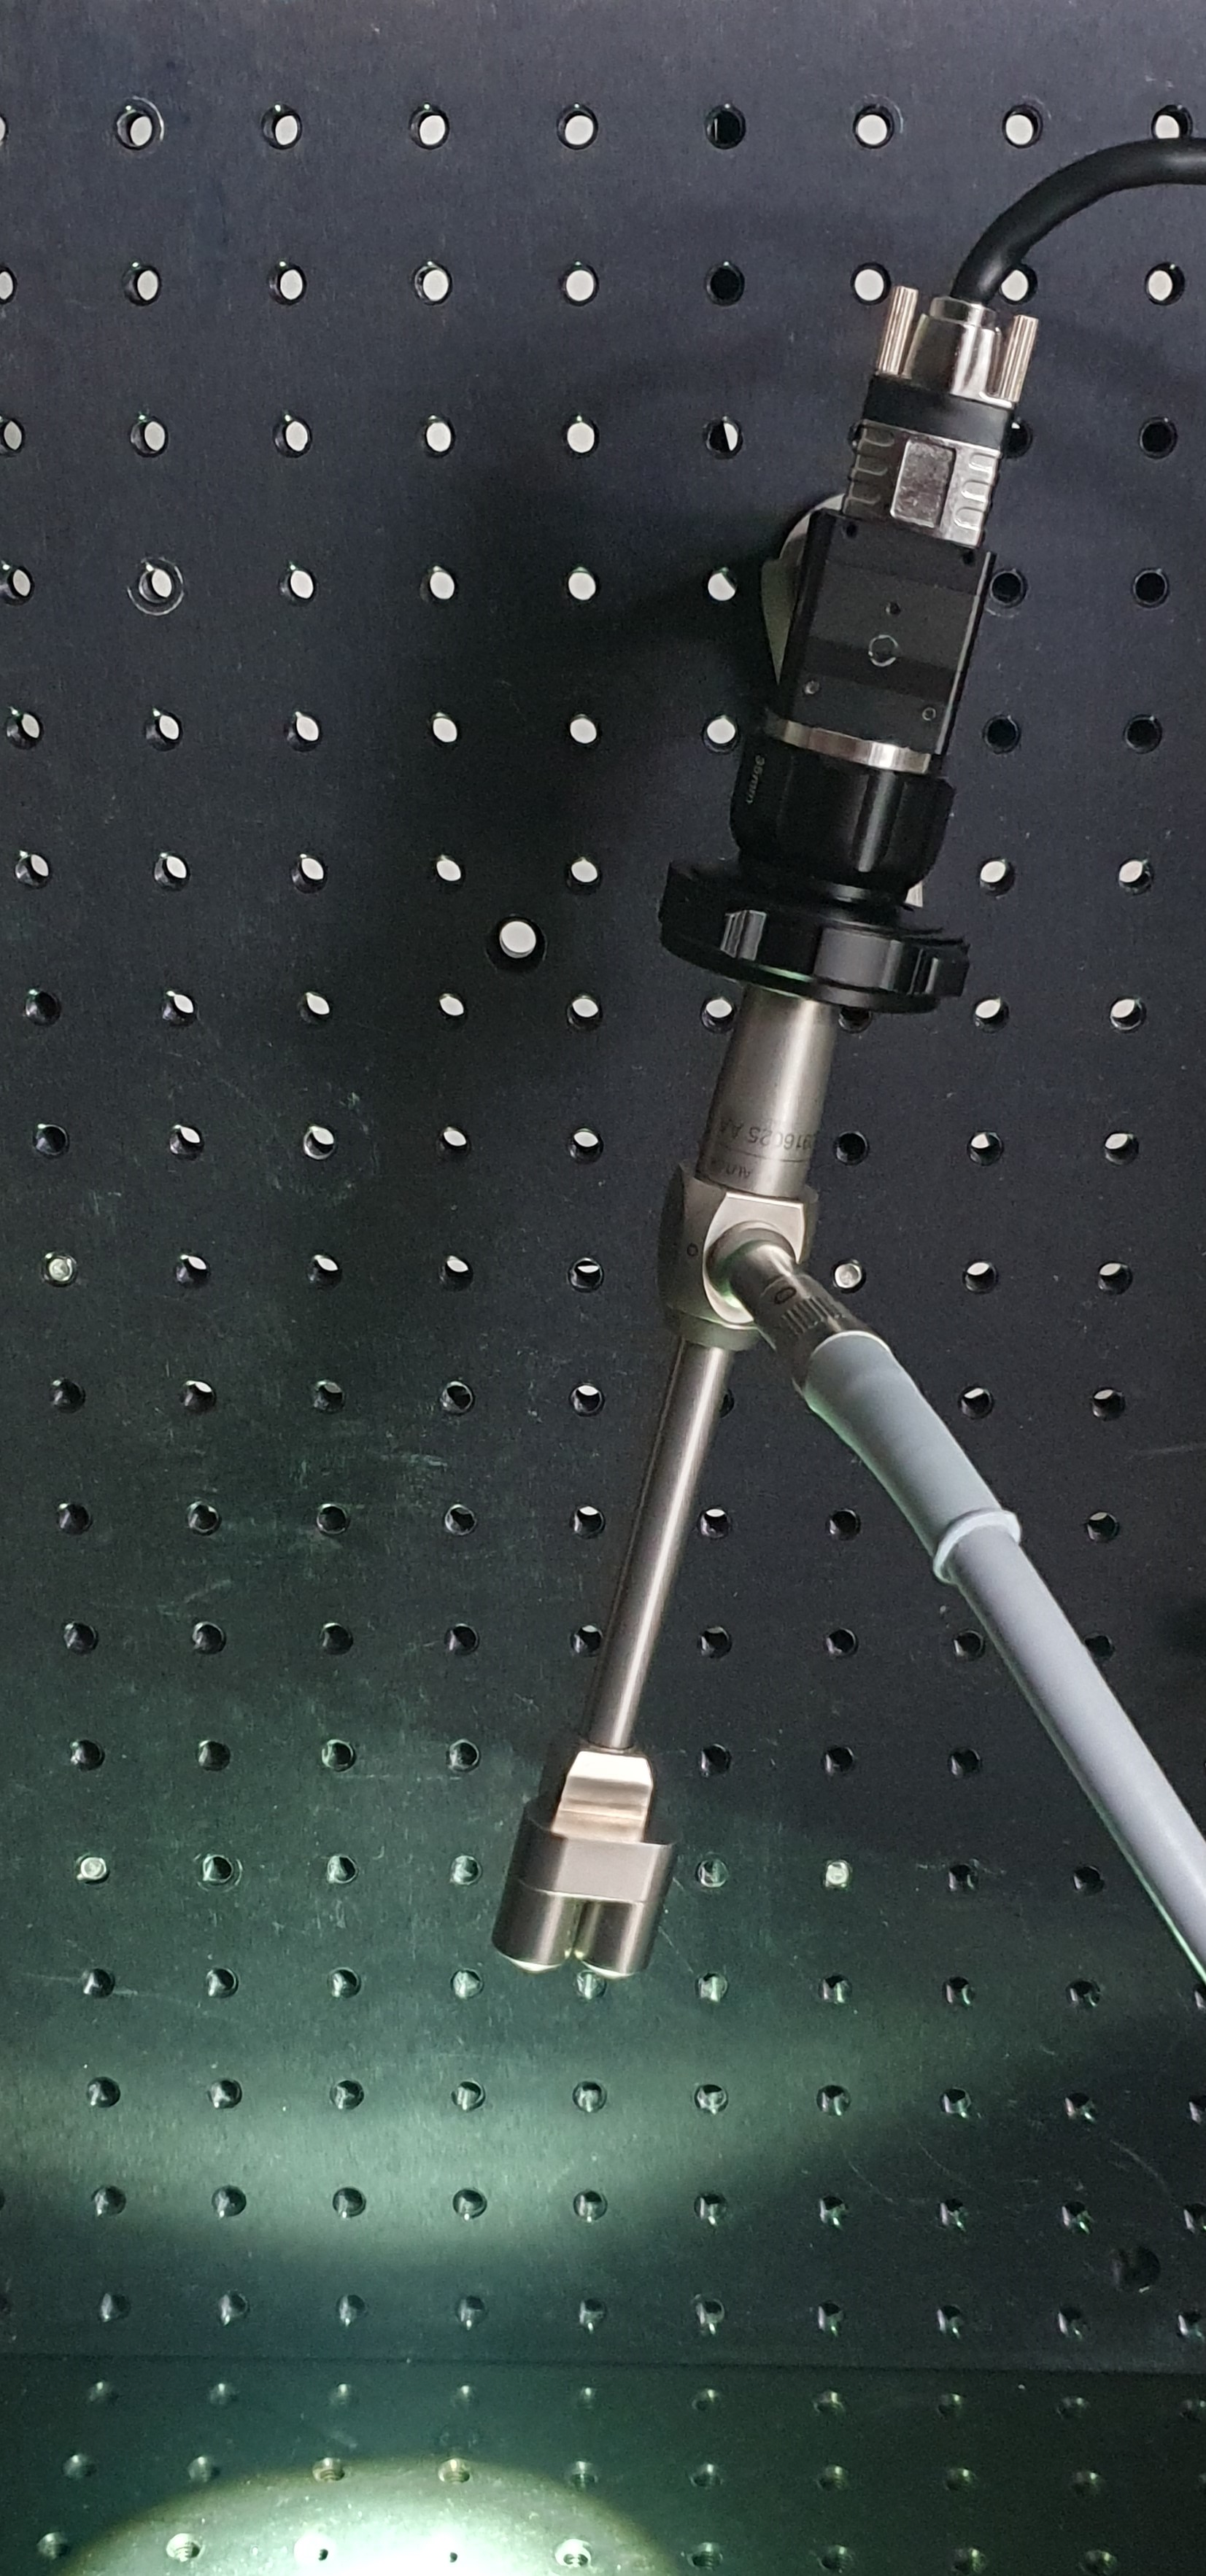
\includegraphics[width=0.3\textwidth]{imagephantoms.jpg}
    \caption{Depiction of hyperspectral imaging set-up used to acquire images of gelatin-based tissue phantoms.}
    \label{fig:imagephantoms}
\end{figure}
The configurations imaged are detailed in Table \ref{tb:imagedphantoms} and cover the majority of the 2-dye configuration dataset that remained viable after two weeks of refrigeration. 
\begin{table}[ht!]
    \centering
    \caption{Table displaying the ratios of dyes [acid red 1 (AR1), acid red 14 (AR14), crystal violet (CV)] a used for each dye configuration alongside the total dye scaled concentration in arbitrary units. The intralipid (v/v \%) imaged for each configuration are also indicated.}
    \begin{tabular}{|c|c|c|c|c|c|c|c|}
        \hline
        Total dye scaled & \multicolumn{2}{|c|}{Dye } & \multicolumn{5}{c|}{Intralipid } \\
        concentration & \multicolumn{2}{|c|}{ratio} & \multicolumn{5}{c|}{concentrations (v/v \%)} \\
        (arbitrary units) & AR1 & AR14 & 1.0 & 2.25 & 3.5 & 4.75 & 6 \\
        \hline
        1 & 1 & 1 & & x & x & x & \\
        10 & 1 & 0 & x & x & x & x & x \\
        10 & 3 & 1 & x & x & x & x & x \\
        10 & 1 & 1 &  & x & x & x & x \\
        10 & 1 & 3 & x & x & x & x & x \\
        10 & 0 & 1 & x & x &  & x & \\
        20 & 1 & 1 &  & & x & x &  \\
        \hline
    \end{tabular}
    \label{tb:imagedphantoms}
\end{table}
A white reference of a Spectralon tile of 95\% is taken under the same lighting conditions and imaging plane as the phantoms. This white reference is either used directly for white balancing quantitative data or to generate spectral sensitivities used to generate mean normalised relative as in Chapter \ref{chap:SWB}. This demonstrates both the highest fidelity and more realistic data processing pathways. Following this, bilinear demosaicing is used and cross-talk correction is applied per pixel of the image also detailed in Chapter \ref{chap:SWB}. 
Each image is manually annotated using ImFusion Labels software to capture pixels corresponding to phantoms while avoiding regions with high specular reflection. This allows a mean spectrum of the phantom to be generated and compared per pixel processing of the annotated region. 

\subsection{Neurosurgical HSI datasets}\label{sec:NeuroHSIdata}
Two neurosurgical HSI datasets are leveraged in this preliminary work. Initially, the HELICoiD dataset is used which captures data in the wavelength range 400-1000nm using a pushbroom spatial scanning HSI camera\cite{Fabelo2019}. This provides 36 images of high spectral resolution which are annotated with use of spectral angle mapper to identify four key classes: "normal tissue, tumor tissue, blood vessel, and background elements". For this work we consider only the spectral range of 450-600nm as this is the range of use for the analytical models considered. Secondly, a NeuroHSI dataset is considered which is obtained using the same snapshot mosaic camera (Ximea utilising the IMEC CMV2K-SSM4X4-VIS sensor, Germany) as in Section \ref{sec:imagingphantoms} whose bands are within the 450-600nm wavelength range. In contrast to Section \ref{sec:imagingphantoms}, this is mounted to a neurosurgical microscope (Zeiss Kinevo 900, Germany) whose integrated light source and lenses are used for simpler integration into the neurosurgical workflow, allowing for use in a wide variety of neurosurgical cases. For each imaging timepoint, the position of the neurosurgical microscope is recorded and used to obtain a flatfield reference outside the sterile field in a closely correlated position and lighting conditions. Similarly to the phantom HSI processing pipeline, this is either used to provide quantitative data from flatfield imaging or used to generate spectral senstivities for relative data before demosaicing and cross-talk correction. These spectral sensitivities are found to be similar to those pre-calculated from the light source spectrum. This dataset is manually annotated using ImFusion Labels software to identify over 30 classes. 

\subsection{Evaluation of analytical models}
The Yudovsky 2009 single and double layer models and Jacques 1999 models are evaluated as these are found to be the most effective in Chapters \ref{chap:1layer} and \ref{chap:2layer}. When using these analytical models with the snapshot HSI datasets outlined in Sections \ref{sec:MCcameras} to \ref{sec:NeuroHSIdata}, the predicted $R$ (detailed in Sections \ref{sec:Jacques}, \ref{sec:Yudovskysingle}, and \ref{sec:Yudovsky2009}) is used to simulate noiseless camera responses as described by Equation \ref{eq:simulatingcam}, however this simulation is not performed for the HELICoiD dataset as the camera band responses are not available and the high spectral resolution limits the deviation from the true spectrum. This allows the forwards and inverse models to be evaluated and quantified as described in Sections \ref{sec:methodevaluate} and \ref{sec:methodevaluate2} against the Monte Carlo datasets, and similarly for the single-layer models for the gelatin-based phantom datsets. For the gelatin-based phantom datasets, either the mean spectrum of the annotated region is used for fitting the inverse model to reduce the impact of noise, or each pixel in the annotated region is used for fitting. The quality of camera simulation can also be evaluated using $NRMSE$ and Pearson correlation coefficients by comparing simulated camera spectra from the spectrophotometer measurements of the gelatin-based phantoms in Section \ref{sec:methodsphantoms}, to the measured HSI data in Section \ref{sec:imagingphantoms}. Finally, for each neurosurgical dataset image, the mean spectrum of each class annotation is calculated and the inverse analytical models are fitted to this. This provides a set of physiological parameters for each class of each image which are then collated to provide a range of values which are evaluated for plausibility. % Need to find better academic phrasing here 
The most effective model is chosen to evaluate an exemplary image on a pixel-by-pixel level with the $StO_2$ values obtained from this displayed alongside the $APE$ from the $StO_2$ values recovered from the mean of the annotated regions in these images. 

\section{Results}

\subsection{Monte Carlo}
The forwards analytical models are assessed using simulated camera responses generated from Monte Carlo data. 
%The Yudovsky 2009 and Jacques 1999 single-layer models are evaluated for three refractive indices, whereas the Yudovsky 2009 double-layer model is evaluated for $n=1.44$ only as in Chapters \ref{chap:1layer} and \ref{chap:2layer}. 
These are evaluated in Table \ref{tb:forwardsHSIMC} for $n=1.44$ (further refractive indices can be found in Appendices \ref{ap:forwardsHSIMCq} and \ref{ap:forwardsHSIMCr}) and examples for the single and double layer configurations shown in Figure \ref{fig:forwardsHSIMC}. 
\begin{table}[h!] %could remove noise levels here
    \centering
    \caption{Mean (standard deviation) $NRMSE$ (3.d.p.) between the simulated camera responses of each forwards spectrum from each model and each of 100 Monte Carlo simulated spectra using the same ground truth variable parameters for quantitative and relative data at a variety of noise levels (0, 0.01, 0.03). This is presented with the Pearson $r$ (bold if Pearson $p < 0.05$) for the linear regression between all forwards spectra against Monte Carlo simulated spectra for each refractive index dataset and each analytical model. All metrics are evaluated for the wavelength region of 450-600nm.}
    \begin{tabular}{|cc|c|ccc|ccc|}
        \hline
        Model & Layers & Quantitative & \multicolumn{3}{|c}{$NRMSE$} & \multicolumn{3}{|c|}{$r$} \\
         & & (Q) or & 0 & 0.01 & 0.03 & 0 & 0.01 & 0.03 \\
         & & Relative (R) &  &  &  &  & &  \\
        \hline
        \multirow{2}{*}{\shortstack{Yudovsky\\ 2009}} & \multirow{2}{*}{1} & Q & \shortstack{0.009 \\(0.004)} & \shortstack{0.082 \\(0.057)} & \shortstack{0.224 \\(0.125)} & \textbf{1.000} & \textbf{0.993} & \textbf{0.942} \\
        & & R & \shortstack{0.003 \\(0.002)} & \shortstack{0.075 \\(0.044)} & \shortstack{0.212 \\(0.118)} & \textbf{1.000} & \textbf{0.916} & \textbf{0.602} \\
        \hline
        \multirow{3}{*}{\shortstack{Jacques\\ 1999}} & \multirow{2}{*}{1} & Q & \shortstack{0.026 \\(0.046)} & \shortstack{0.089 \\(0.077)} & \shortstack{0.227 \\(0.130)} & \textbf{1.000} & \textbf{0.993} & \textbf{0.942} \\
        & & R & \shortstack{0.014 \\(0.021)} & \shortstack{0.076 \\(0.045)} & \shortstack{0.212 \\(0.117)} & \textbf{0.995} & \textbf{0.915} & \textbf{0.605} \\
        \hline
        \multirow{2}{*}{\shortstack{Yudovsky\\ 2009}} & \multirow{2}{*}{2} & Q & \shortstack{0.166 \\(0.133)} & \shortstack{0.482 \\(0.289)} & \shortstack{0.738 \\(0.294)} & \textbf{0.992} & \textbf{0.971} & \textbf{0.829} \\
         &  & R & \shortstack{0.033 \\(0.026)} & \shortstack{0.428 \\(0.286)} & \shortstack{0.684 \\(0.286)} & \textbf{0.991} & \textbf{0.270} & -0.007 \\
        \hline
    \end{tabular}
    \label{tb:forwardsHSIMC}
\end{table}

\begin{figure}[h!]
    \centering
    \begin{subfigure}{0.49\textwidth}
        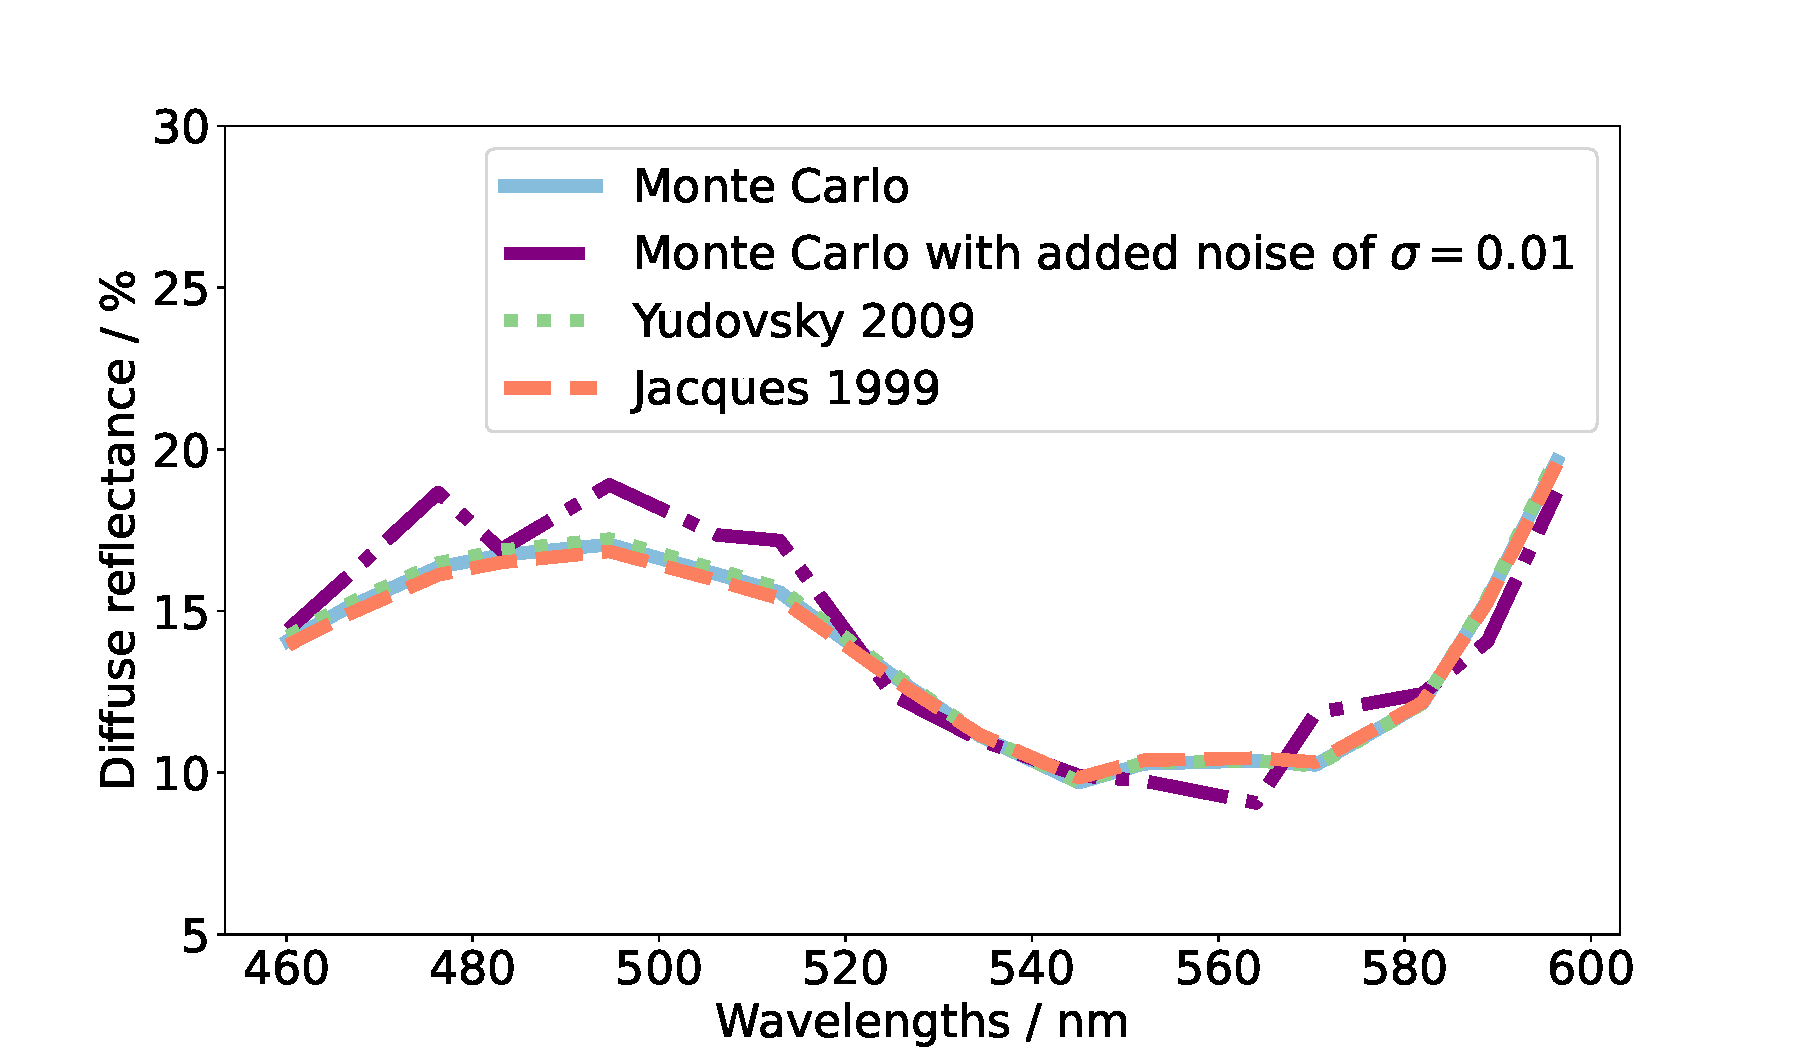
\includegraphics[width=\textwidth]{forwards_noise_Q.pdf}
        \caption{}
        \label{fig:egforwardsnoiseQ}
    \end{subfigure}
    \begin{subfigure}{0.49\textwidth}
        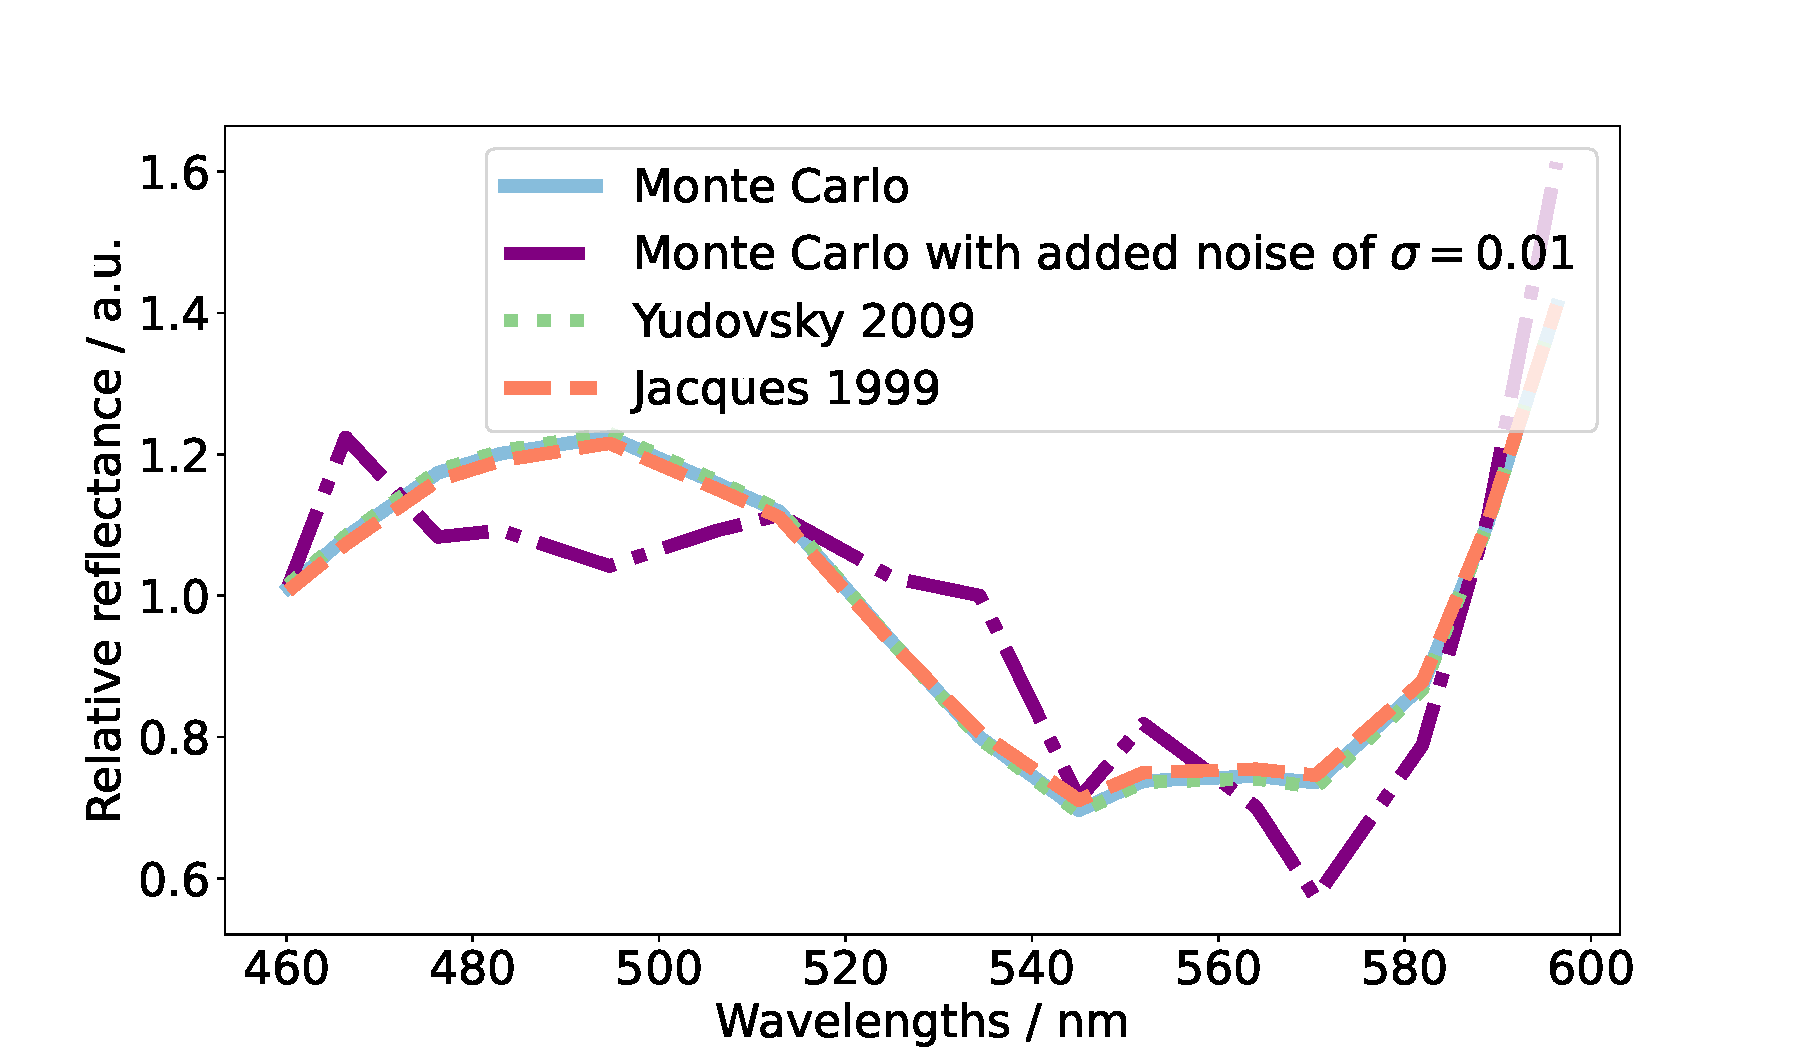
\includegraphics[width=\textwidth]{forwards_noise_R.pdf}
        \caption{}
        \label{fig:egforwardsnoiseR}
    \end{subfigure}
    \begin{subfigure}{0.49\textwidth}
        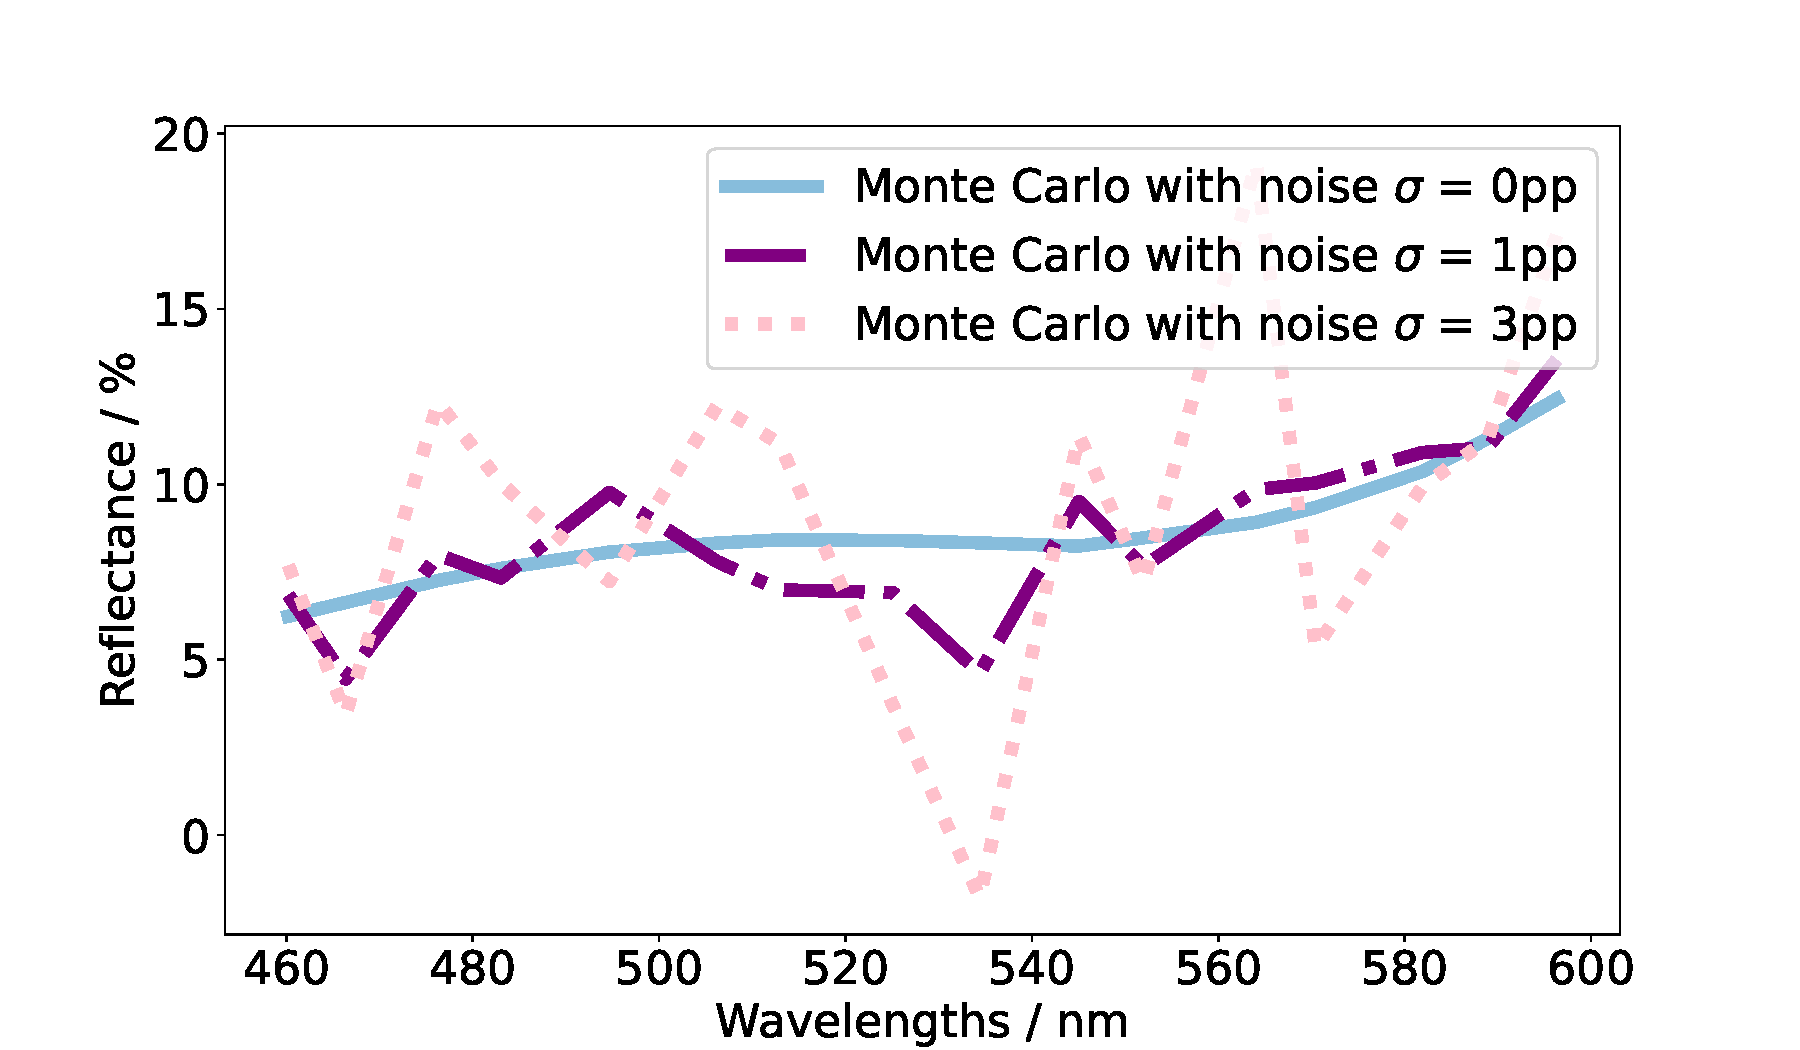
\includegraphics[width=\textwidth]{forwards_noise2_Q.pdf}
        \caption{}
        \label{fig:egforwards2noiseQ}
    \end{subfigure}
    \begin{subfigure}{0.49\textwidth}
        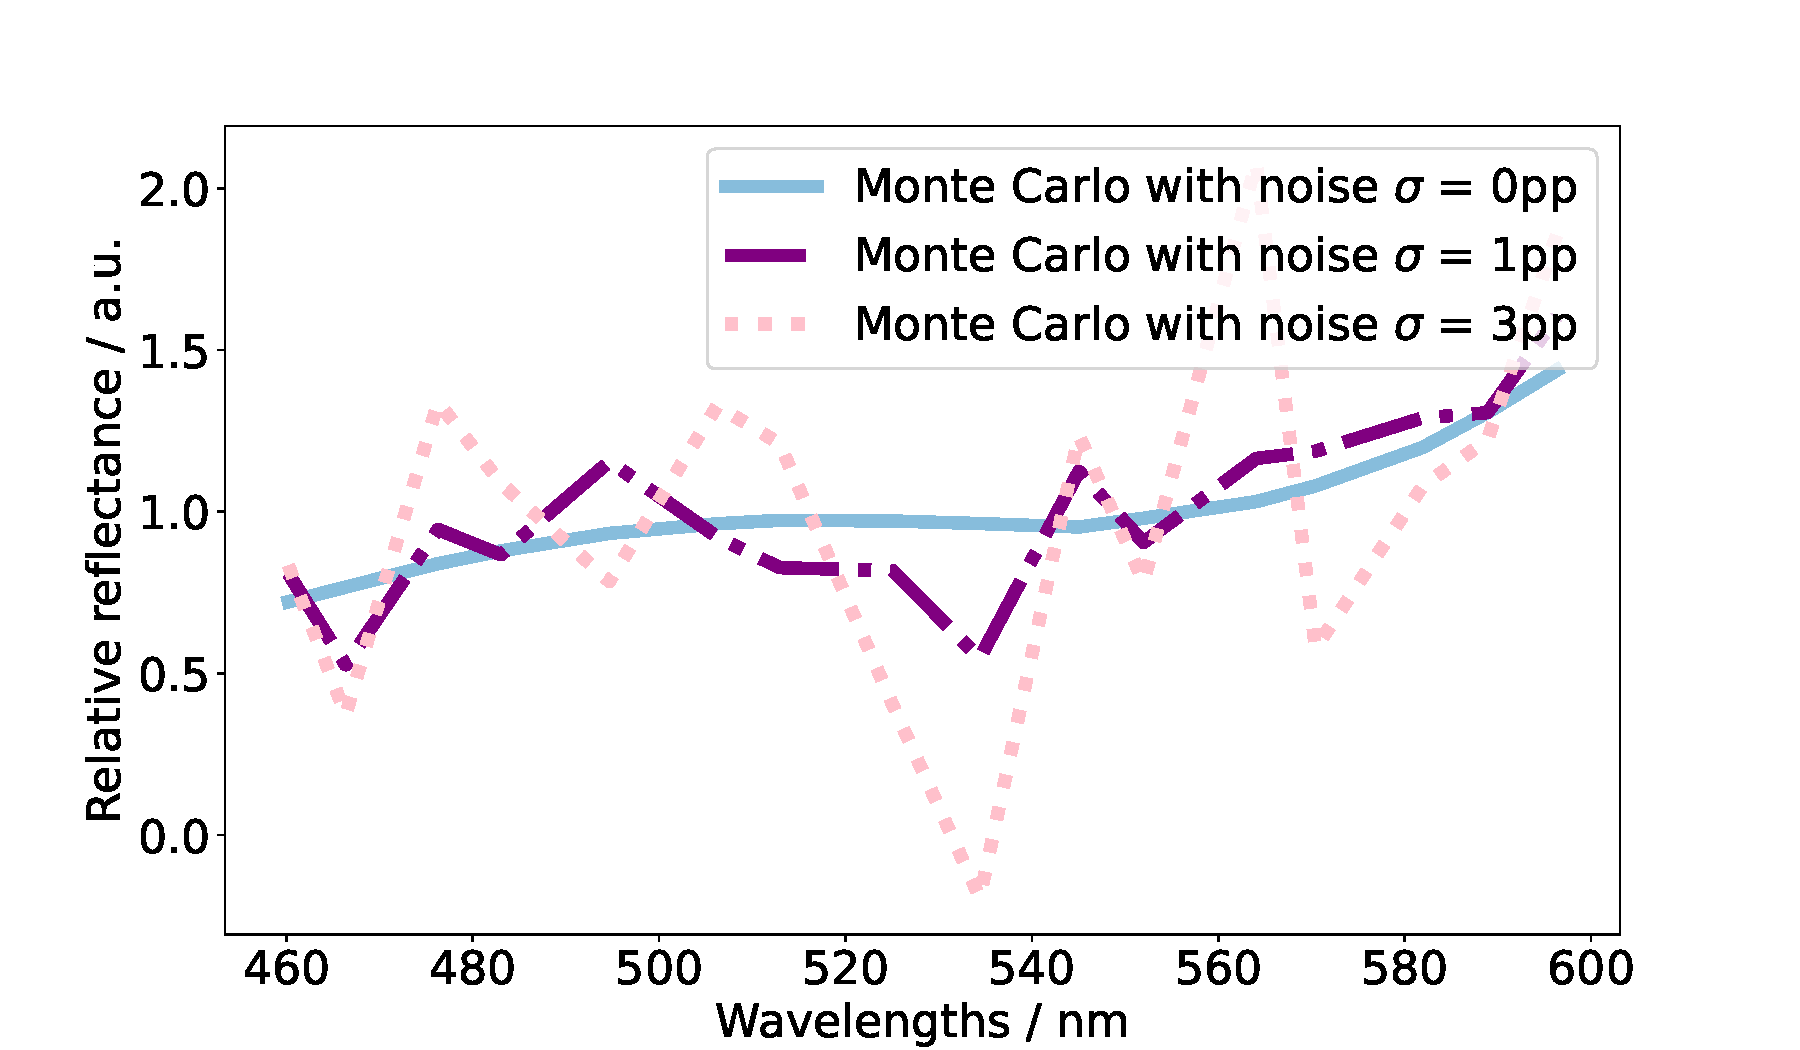
\includegraphics[width=\textwidth]{forwards_noise2_R.pdf}
        \caption{}
        \label{fig:egforwards2noiseR}
    \end{subfigure}
    \caption{Top: Example of the simulated camera response spectra from each forward single-layer analytical model: Yudovsky 2009 (\textcolor{MyGreen}{green dotted}) and Jacques 1999 (\textcolor{MyOrange}{orange dashed}), using ground truth variables for a refractive index of 1.44 compared to that predicted by Monte Carlo with (\textcolor{purple}{purple dash-dotted} and without noise added (\textcolor{MyBlue}{blue solid}) for quantitative (left) and relative (right) data. Bottom: Demonstration of the variability of quality of prediction between the simulated camera responses from the Yudovsky 2009 two layer model (\textcolor{MyGreen}{green dotted}) and Monte Carlo with (\textcolor{purple}{purple dash-dotted} and without noise added (\textcolor{MyBlue}{blue solid}) when using the same ground truth parameters for quantitative (left) or relative (right) data.}
    \label{fig:forwardsHSIMC}
\end{figure}

The inverse models are fitted to these varying noise level datasets and the evaluation of these results can be seen in Table \ref{tb:backwardsHSIMC} for $n=1.44$ (with further refractive indices in Appendices \ref{ap:backwardsHSIMCq} and \ref{ap:backwardsHSIMCr}) and examples of the $StO_2$ extraction quality in Figure \ref{fig:backwardsHSIMC1} for single-layer models and Figure \ref{fig:backwardsHSIMC2} for the double-layer model. 

\begin{table}[h!]
    \centering
    \caption{The Pearson $r$ values (bold if $p<0.05$) of the linear regression line between the fitted tissue parameters and their ground truth displayed with their median absolute percentage errors ($APE$). This is shown for each variable when extracted by fitting Yudovsky 2009 single layer (Y1), Jacques 1999 (J), or Yudovsky 2009 double layer (Y2) to the quantitative (Q) or relative (R) Monte-Carlo datasets for $n=1.44$ at each noise level (0, 0.01, 0.03). All presented to 3s.f.}
    \begin{tabular}{|ccc|ccc|ccc|}
        \hline
        Parameter & Model & Quantitative & \multicolumn{3}{c}{$r$} & \multicolumn{3}{|c|}{median} \\
        & & (Q) or & \multicolumn{3}{c}{} & \multicolumn{3}{|c|}{$APE$ (\%)} \\
        & & Relative (R) & 0 & 0.01 & 0.03 & 0 & 0.01 & 0.03 \\
        \hline
        \multirow{6}{*}{$StO_2$} & \multirow{2}{*}{Y1} & Q & \textbf{0.999} & \textbf{0.825} & \textbf{0.369} & 1.90 & 24.8 & 85.2 \\
        & & R & \textbf{0.999} & \textbf{0.752} & \textbf{0.410} & 2.23 & 41.4 & 76.7 \\
        \cline{2-9}
        & \multirow{2}{*}{J} & Q & \textbf{0.978} & \textbf{0.829} & \textbf{0.402} & 4.06 & 22.5 & 83.6 \\
        & & R & \textbf{0.977} & \textbf{0.755} & \textbf{0.447} & 4.77 & 40.3 & 76.7 \\
        \cline{2-9}
        & \multirow{2}{*}{Y2} & Q & \textbf{0.751} & 0.0612 & 0.0194 & 16.8 & 66.5 & 68.9 \\
        & & R & \textbf{0.679} & \textbf{0.198} & 0.0448 & 18.8 & 63.0 & 75.1 \\
        \hline
        \multirow{6}{*}{$f_{blood}$} & \multirow{2}{*}{Y1} & Q & \textbf{0.984} & \textbf{0.667} & \textbf{0.450} & 5.83 & 23.7 & 51.8\\
        & & R & \textbf{0.870} & \textbf{0.547} & \textbf{0.535} & 16.7 & 47.5 & 51.1\\
        \cline{2-9}
        & \multirow{2}{*}{J} & Q & \textbf{0.924} & \textbf{0.719} & \textbf{0.498} & 7.14 & 25.0 & 46.7 \\
        & & R & \textbf{0.859} & \textbf{0.681} & \textbf{0.644} & 24.1 & 39.6 & 45.0 \\
        \cline{2-9}
        & \multirow{2}{*}{Y2} & Q & \textbf{0.872} & 0.147 & 0.0329 & 23.1 & 115 & 160 \\
        & & R & \textbf{0.609} & 0.189 & 0.0466 & 37.6 & 97.7 & 108 \\
        \hline
        \multirow{6}{*}{$a$} & \multirow{2}{*}{Y1} & Q & \textbf{0.992} & \textbf{0.773} & \textbf{0.558} & 3.85 & 18.7 & 35.1 \\
        & & R & \textbf{0.703} & 0.160 & \textbf{0.558} & 26.2 & 62.3 & 35.1 \\
        \cline{2-9}
        & \multirow{2}{*}{J} & Q & \textbf{0.961} & \textbf{0.759} & \textbf{0.542} & 4.69 & 17.1 & 30.4 \\
        & & R & \textbf{0.431} & -0.00356 & 0.166 & 27.7 & 57.7 & 51.7 \\
        \cline{2-9}
        & \multirow{2}{*}{Y2} & Q & \textbf{0.674} & 0.00365 & 0.0666 & 17.9 & 37.8 & 37.4 \\
        & & R & \textbf{0.333} & 0.0199 & -0.100 & 27.0 & 36.7 & 42.2 \\
        \hline
        \multirow{6}{*}{$b$} & \multirow{2}{*}{Y1} & Q & \textbf{0.998} & \textbf{0.751} & \textbf{0.516} & 2.63 & 21.8 & 52.0 \\
        & & R & \textbf{0.996} & \textbf{0.607} & \textbf{0.426} & 3.31 & 39.5 & 51.2 \\
        \cline{2-9}
        & \multirow{2}{*}{J} & Q & \textbf{0.934} & \textbf{0.757} & \textbf{0.515} & 5.70 & 23.7 & 50.4 \\
        & & R & \textbf{0.938} & \textbf{0.641} & \textbf{0.441} & 7.66 & 32.6 & 46.4 \\
        \cline{2-9}
        & \multirow{2}{*}{Y2} & Q & \textbf{0.735} & 0.169 & -0.00249 & 16.8 & 56.4 & 61.3 \\
        & & R & \textbf{0.360} & 0.0441 & -0.0711 & 33.2 & 61.7 & 63.6 \\
        \hline
        \multirow{2}{*}{$f_{mel}$} & \multirow{2}{*}{Y2} & Q & \textbf{0.852} & \textbf{0.622} & \textbf{0.477} & 28.0 & 85.1 & 90.1 \\ 
        & & R & \textbf{0.517} & 0.166 & \textbf{0.201} & 35.3 & 108 & 132 \\
        \hline
        \multirow{2}{*}{$L_1$} & \multirow{2}{*}{Y2} & Q & \textbf{0.824} & \textbf{0.401} & 0.123 & 36.7 & 69.5 & 84.5 \\
        & & R & \textbf{0.806} & 0.0777 & -0.0675 & 38.1 & 65.4 & 76.6 \\
        \hline
    \end{tabular}    
    \label{tb:backwardsHSIMC}
\end{table}

%could reduce number of things shown below/put some in supplementary but unsure
\begin{figure}[h!]
    \centering
    \begin{subfigure}{0.49\textwidth}
        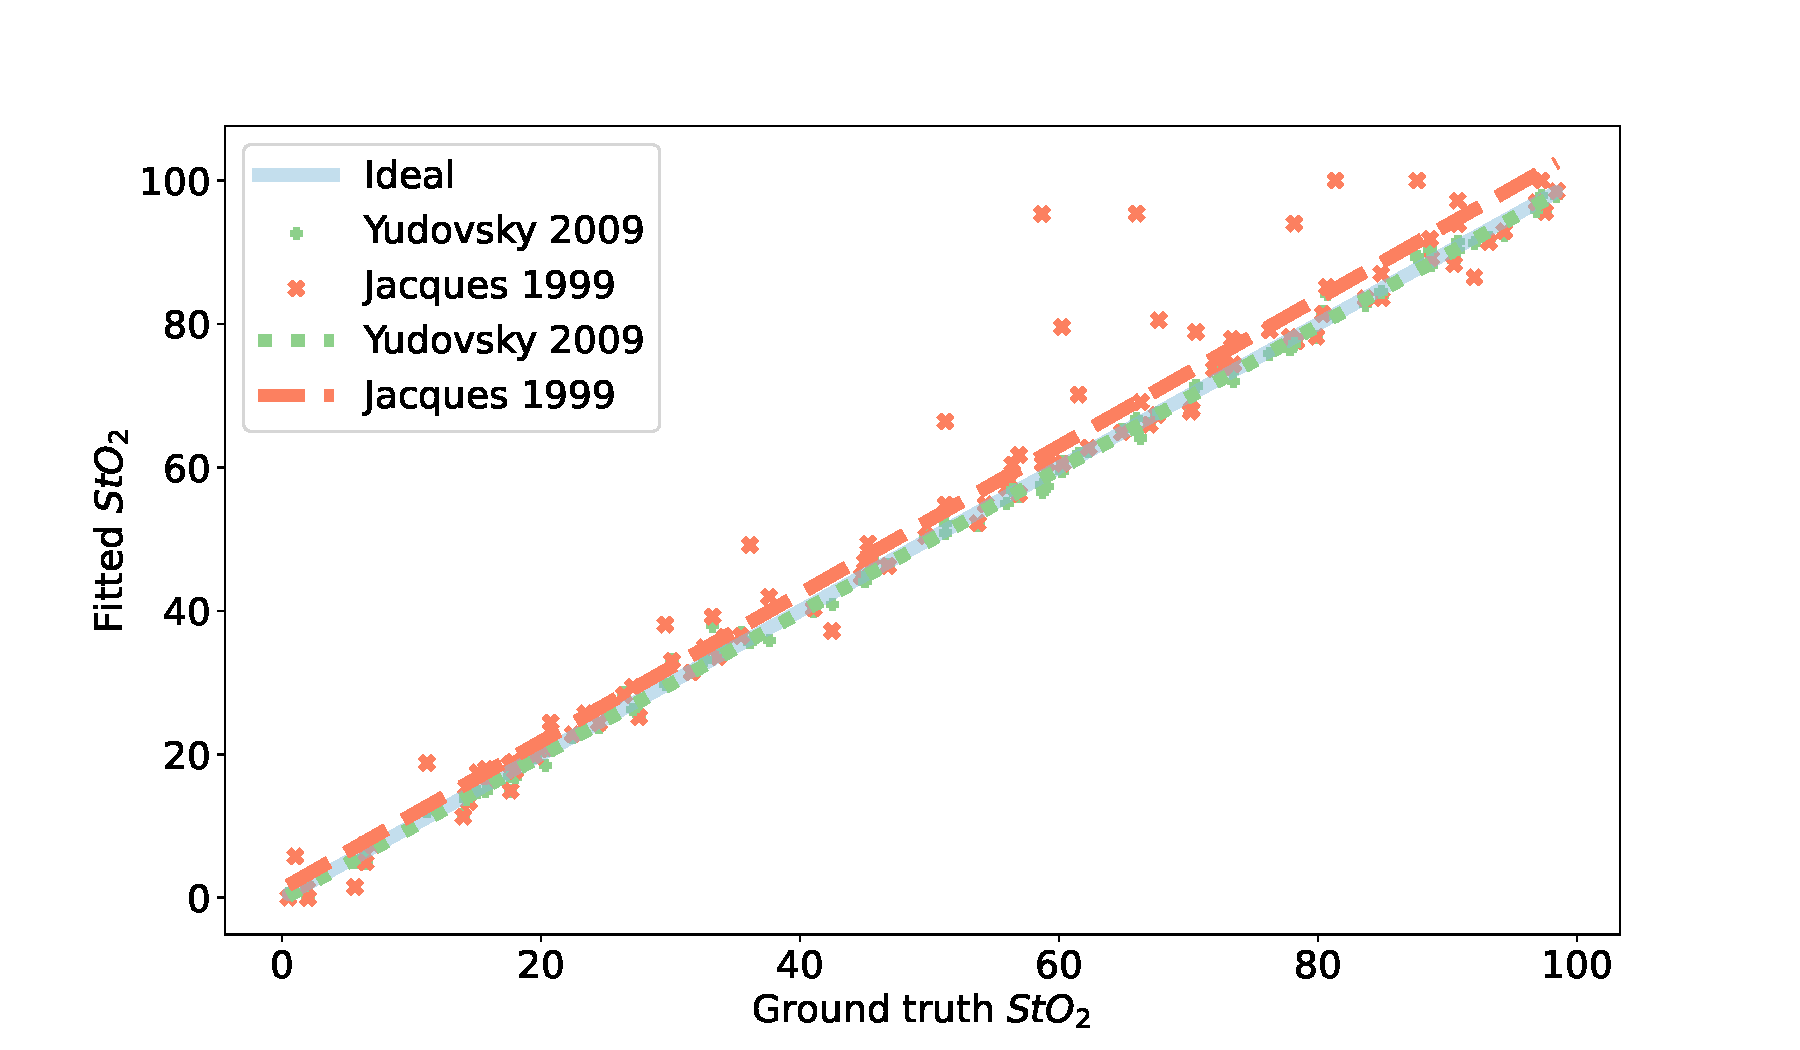
\includegraphics[width=\textwidth]{backwardsn0Q.pdf}
        \caption{}
        \label{fig:backwardsn0Q}
    \end{subfigure}
    \begin{subfigure}{0.49\textwidth}
        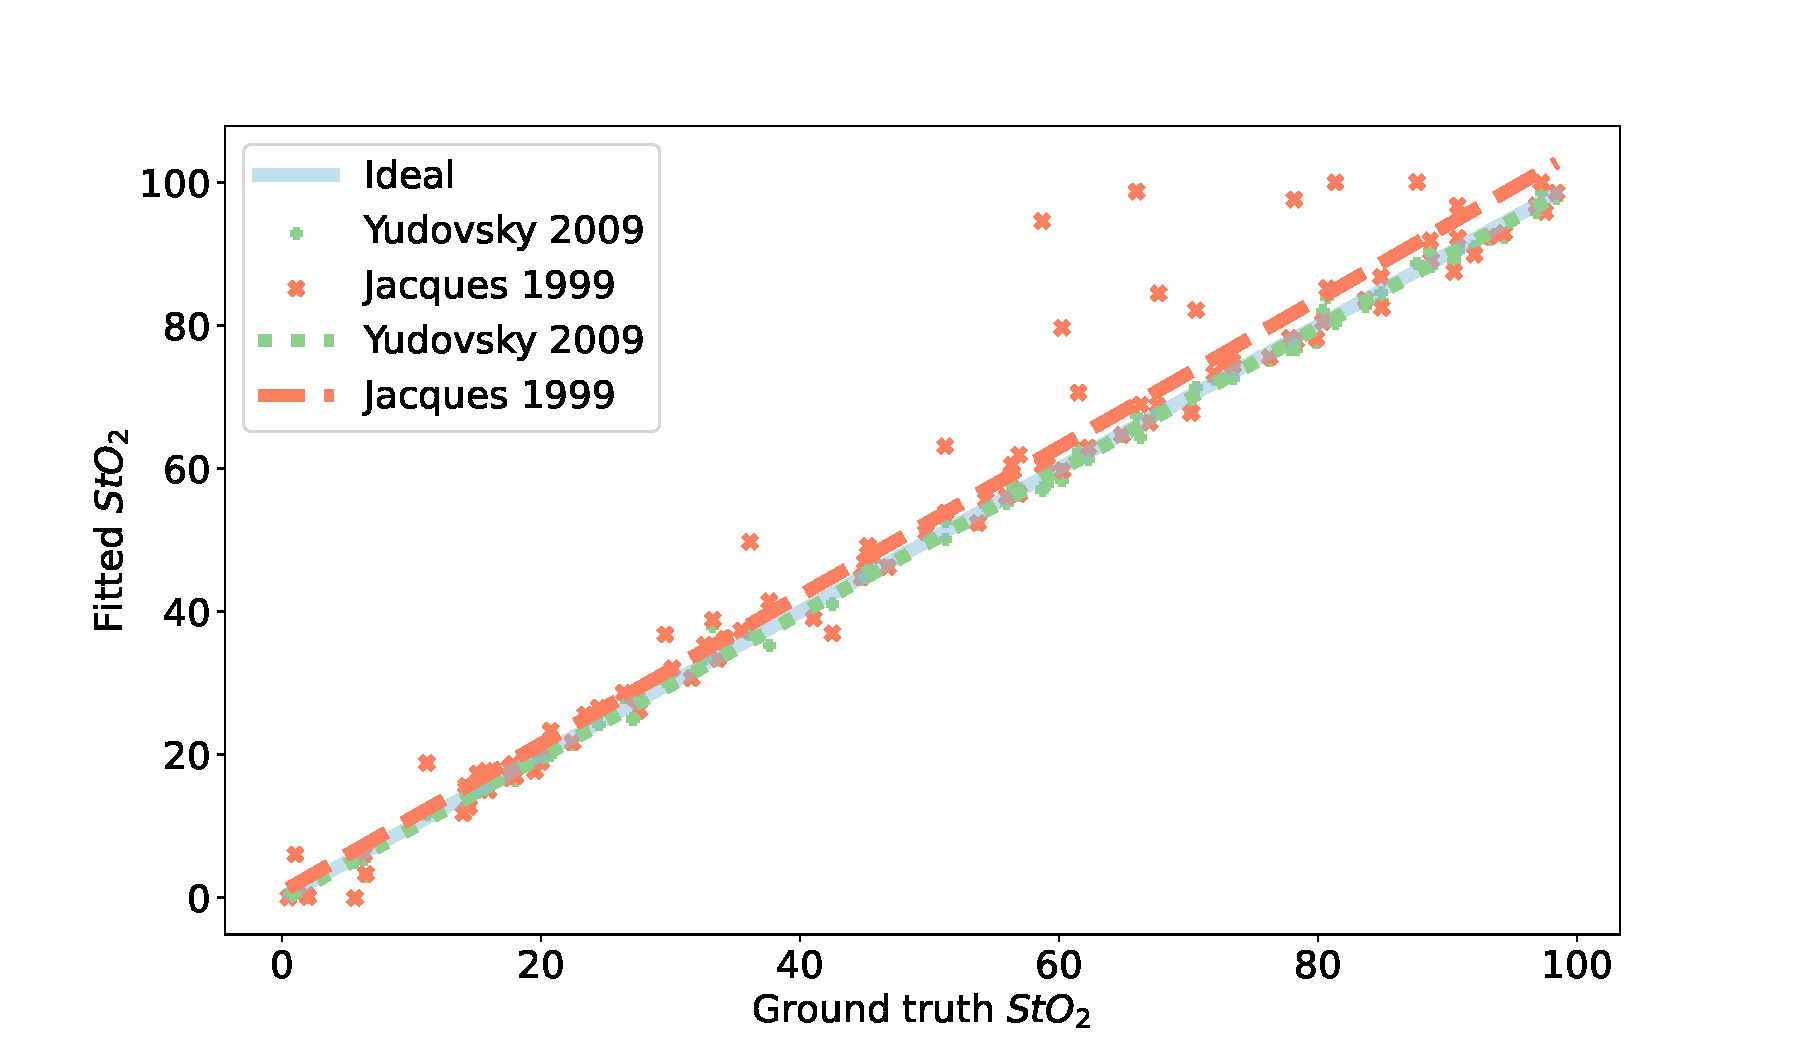
\includegraphics[width=\textwidth]{backwardsn0R.pdf}
        \caption{}
        \label{fig:backwardsn0R}
    \end{subfigure}
    \begin{subfigure}{0.49\textwidth}
        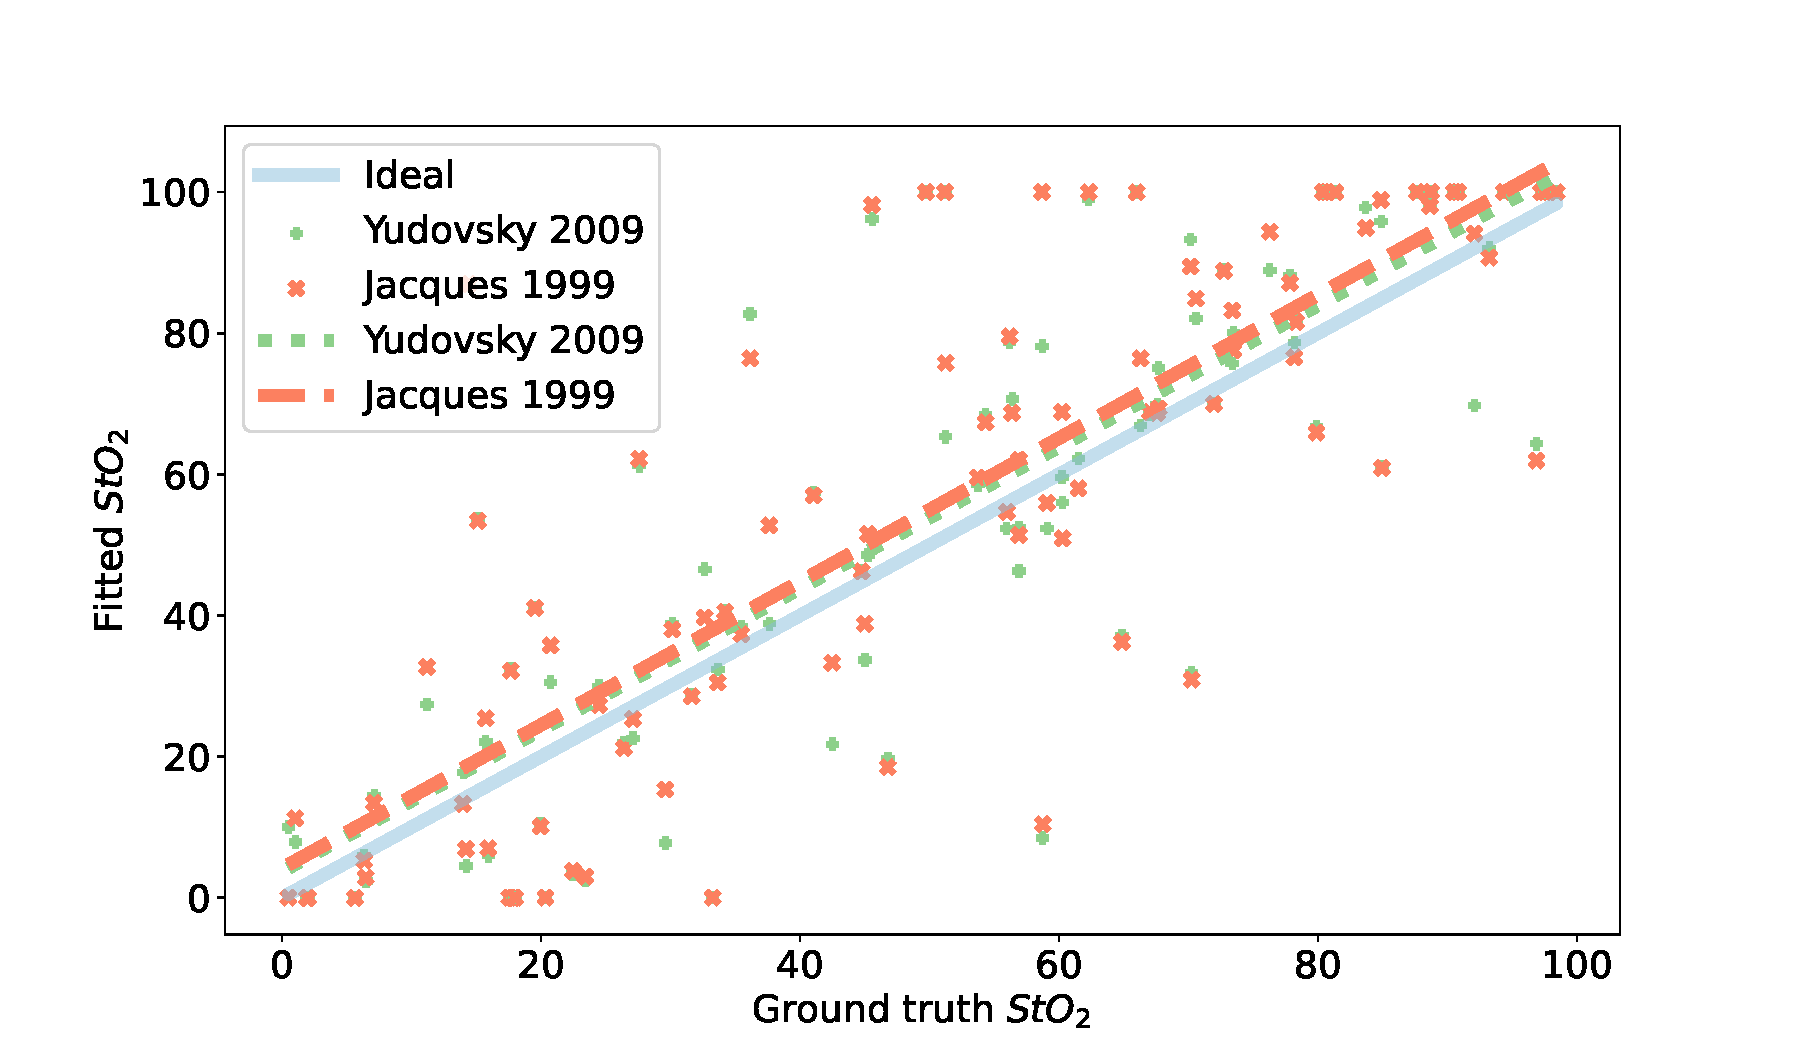
\includegraphics[width=\textwidth]{backwardsn0.01Q.pdf}
        \caption{}
        \label{fig:backwardsn0.01Q}
    \end{subfigure}
    \begin{subfigure}{0.49\textwidth}
        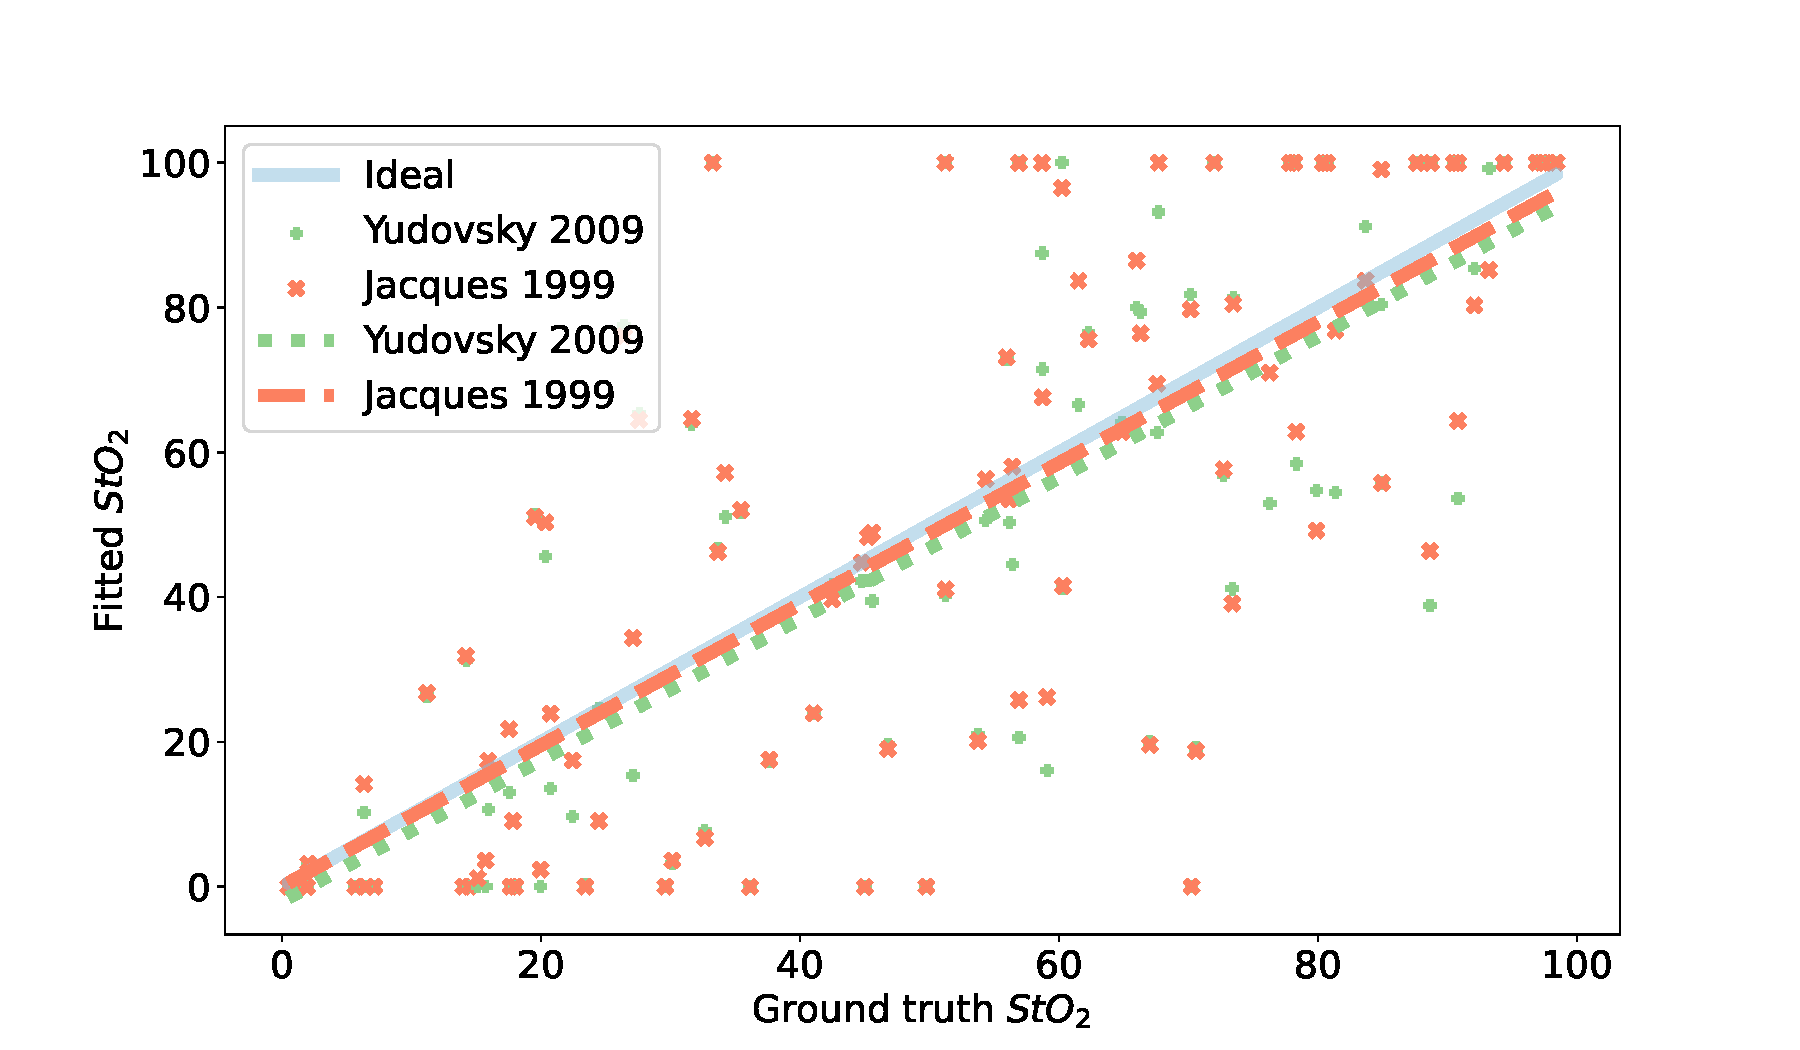
\includegraphics[width=\textwidth]{backwardsn0.01R.pdf}
        \caption{}
        \label{fig:backwardsm0.01R}
    \end{subfigure}
    \begin{subfigure}{0.49\textwidth}
        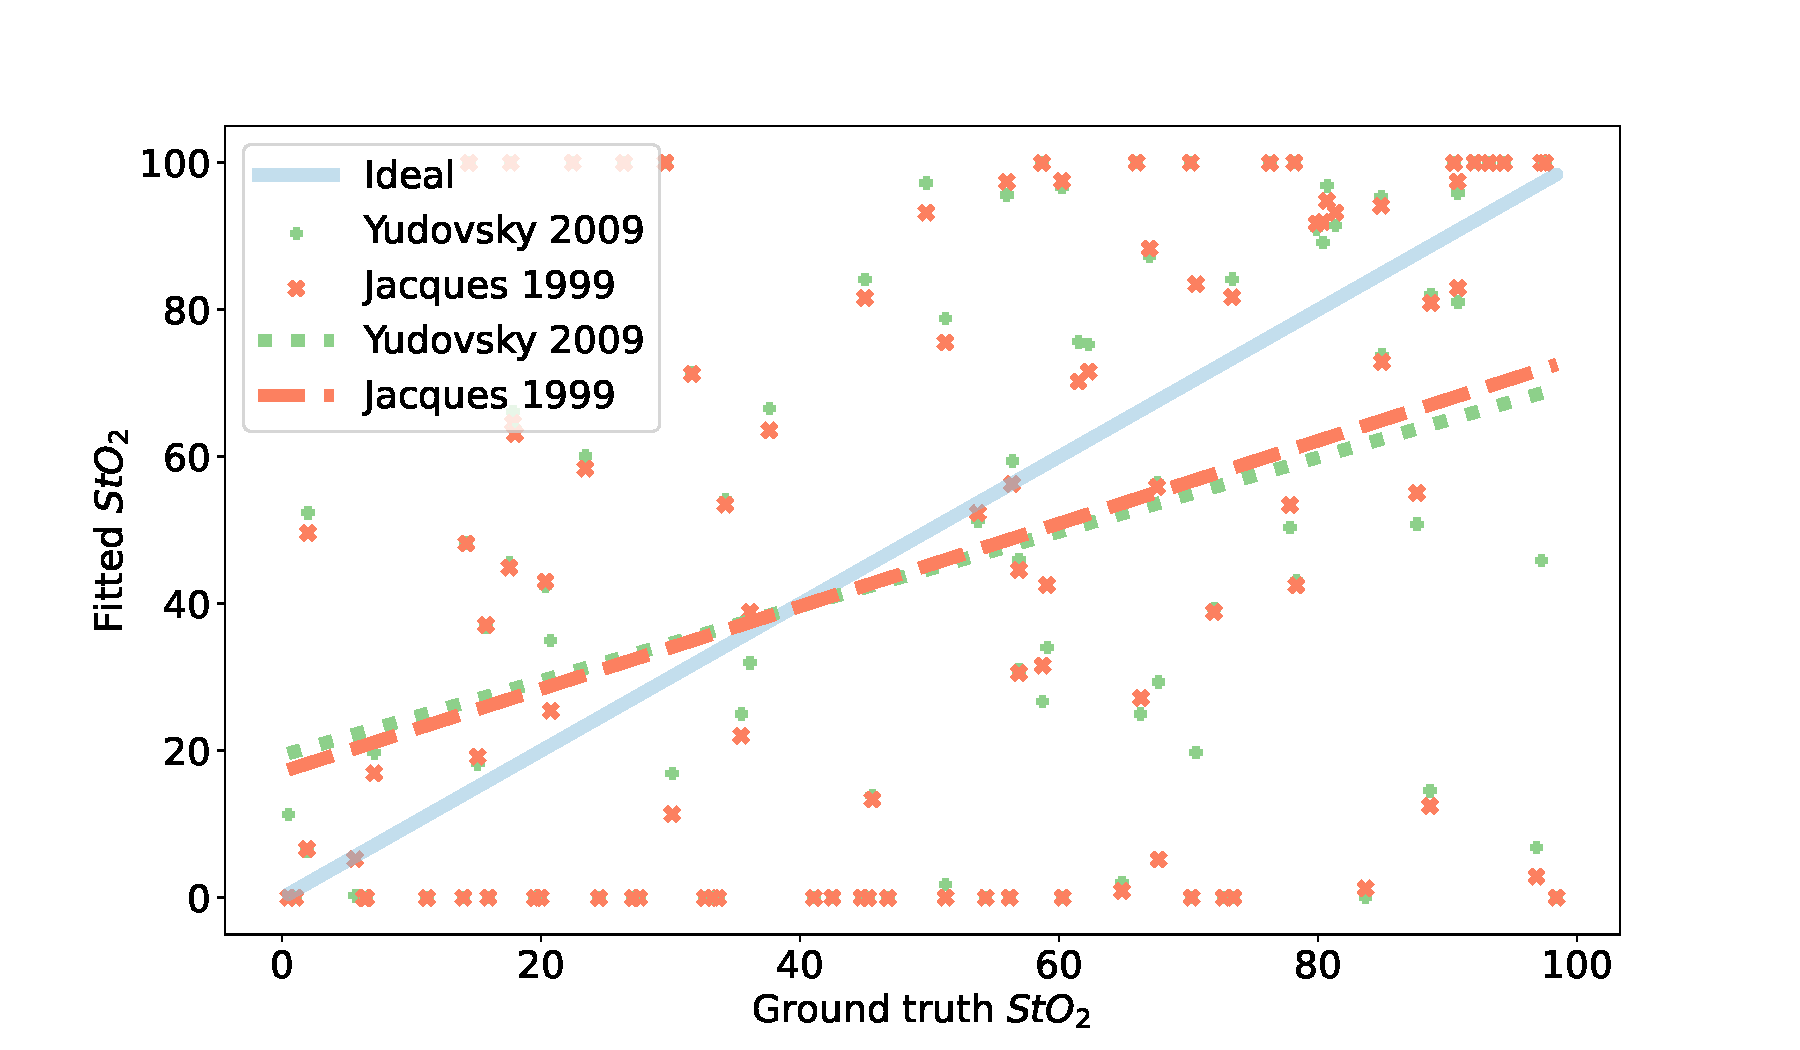
\includegraphics[width=\textwidth]{backwardsn0.03Q.pdf}
        \caption{}
        \label{fig:backwardsn0.03Q}
    \end{subfigure}
    \begin{subfigure}{0.49\textwidth}
        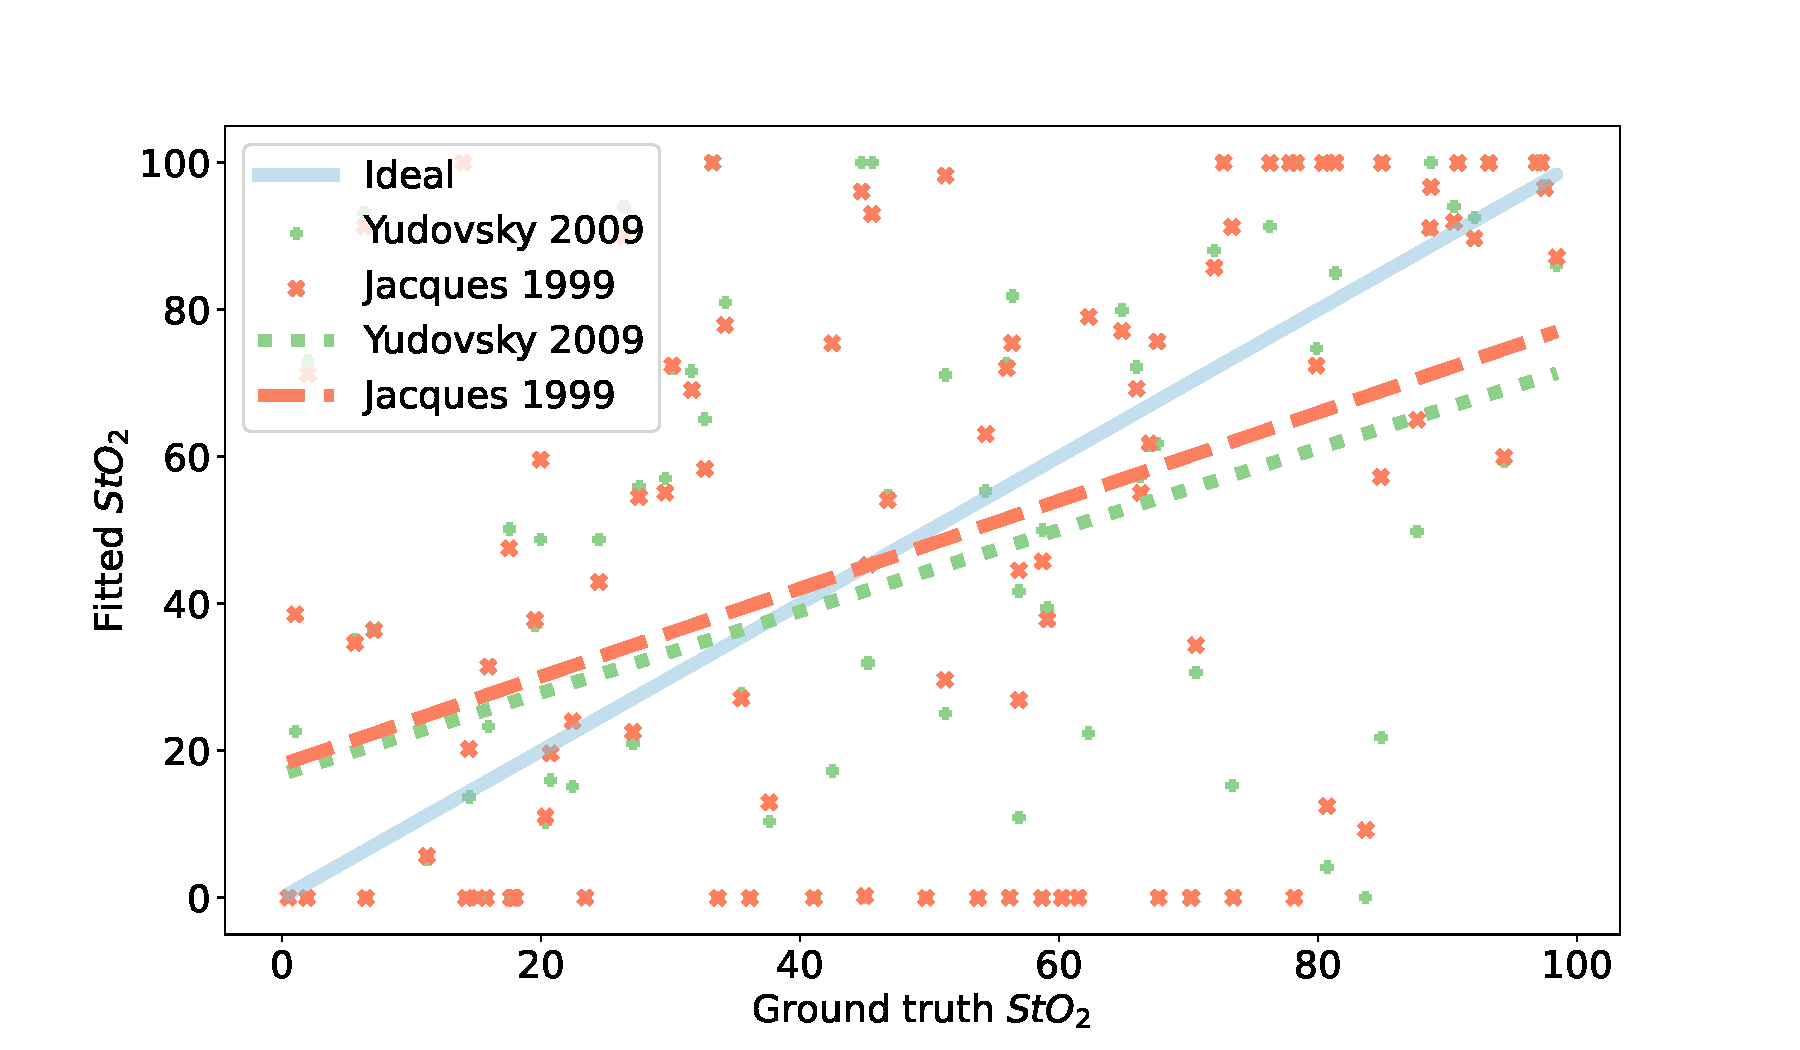
\includegraphics[width=\textwidth]{backwardsn0.03R.pdf}
        \caption{}
        \label{fig:backwardsm0.03R}
    \end{subfigure}
    \caption{An example of the quality of parameter recovery by fitting each inverse analytical model (Yudovsky 2009 (\textcolor{MyGreen}{green $+$}) and Jacques 1999 (\textcolor{MyOrange}{orange $\times$})) to the quantitative (left) or relative (right) simulated camera responses from the Monte Carlo simulations and their associated trend lines for a refractive index of 1.44 for $StO_2$. This is shown for data with either no added noise (top) or added noise with $\sigma = 0.01$ (middle) or $\sigma = 0.03$ (bottom).}
    \label{fig:backwardsHSIMC1}
\end{figure}

\begin{figure}[h!]
    \centering
    \begin{subfigure}{0.49\textwidth}
        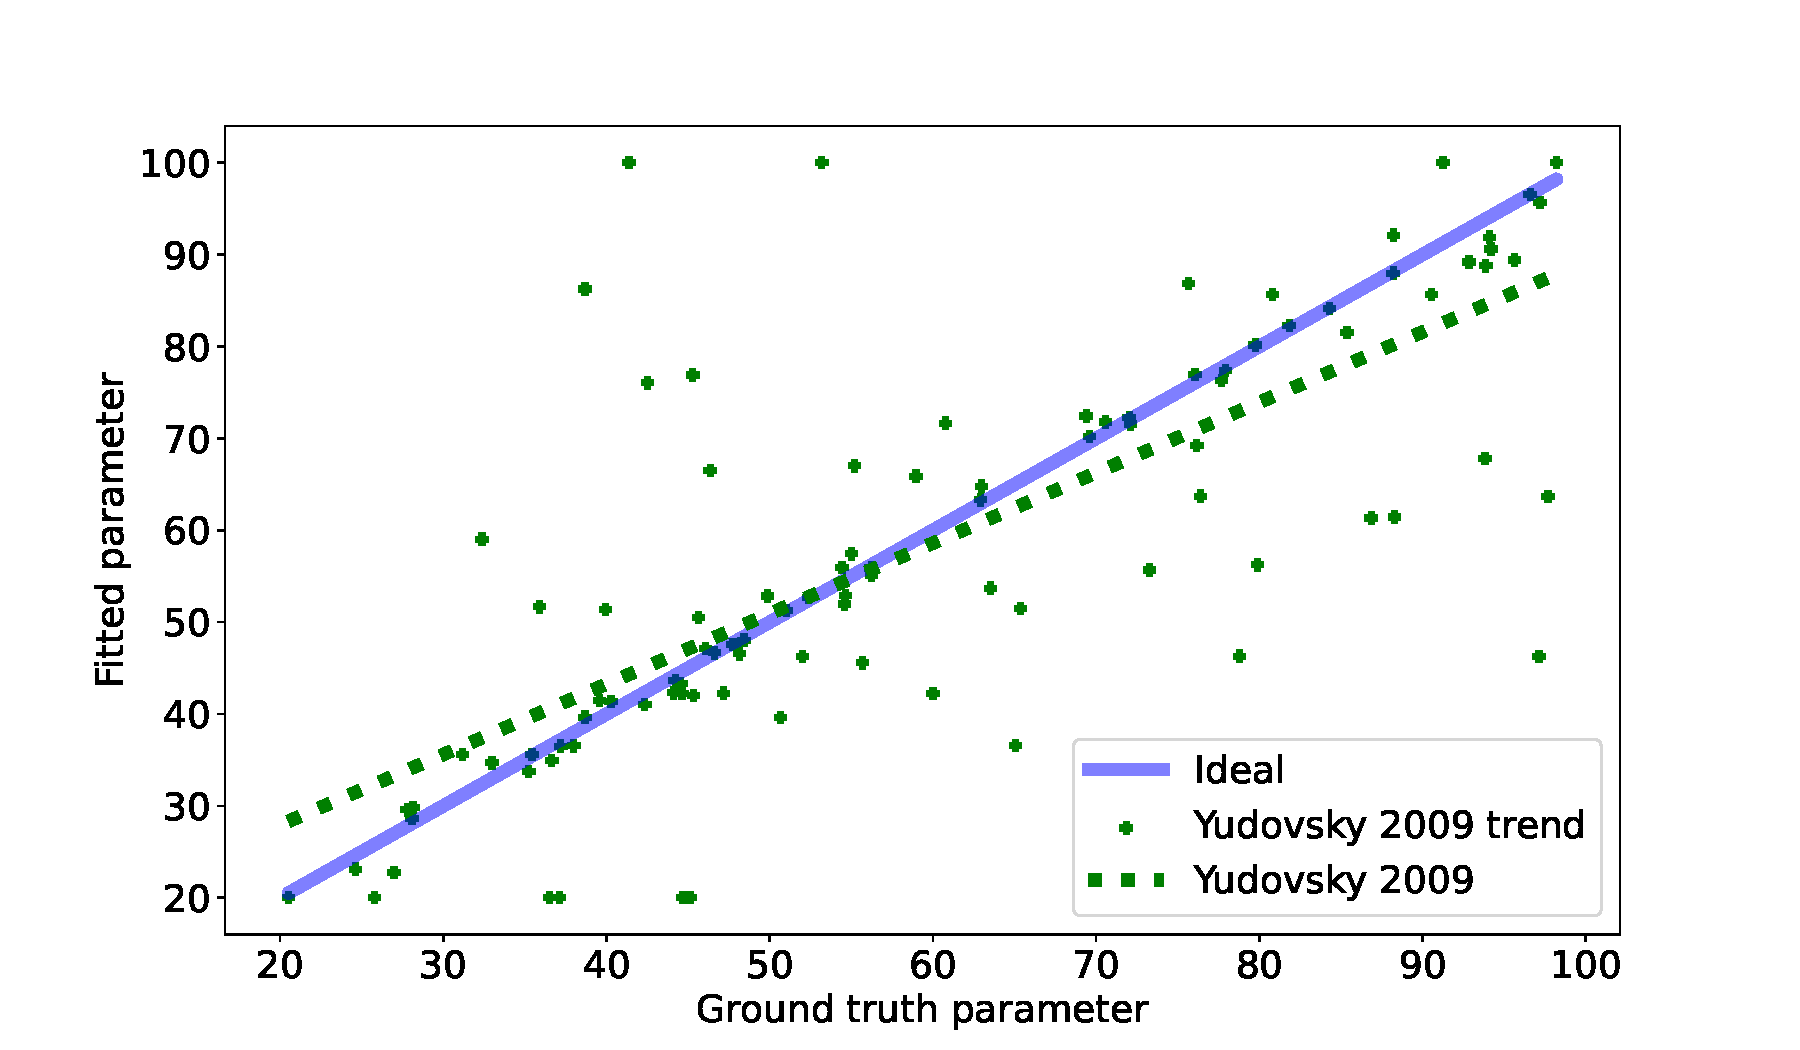
\includegraphics[width=\textwidth]{backwardsn0Q2.pdf}
        \caption{}
        \label{fig:backwardsn0Q2}
    \end{subfigure}
    \begin{subfigure}{0.49\textwidth}
        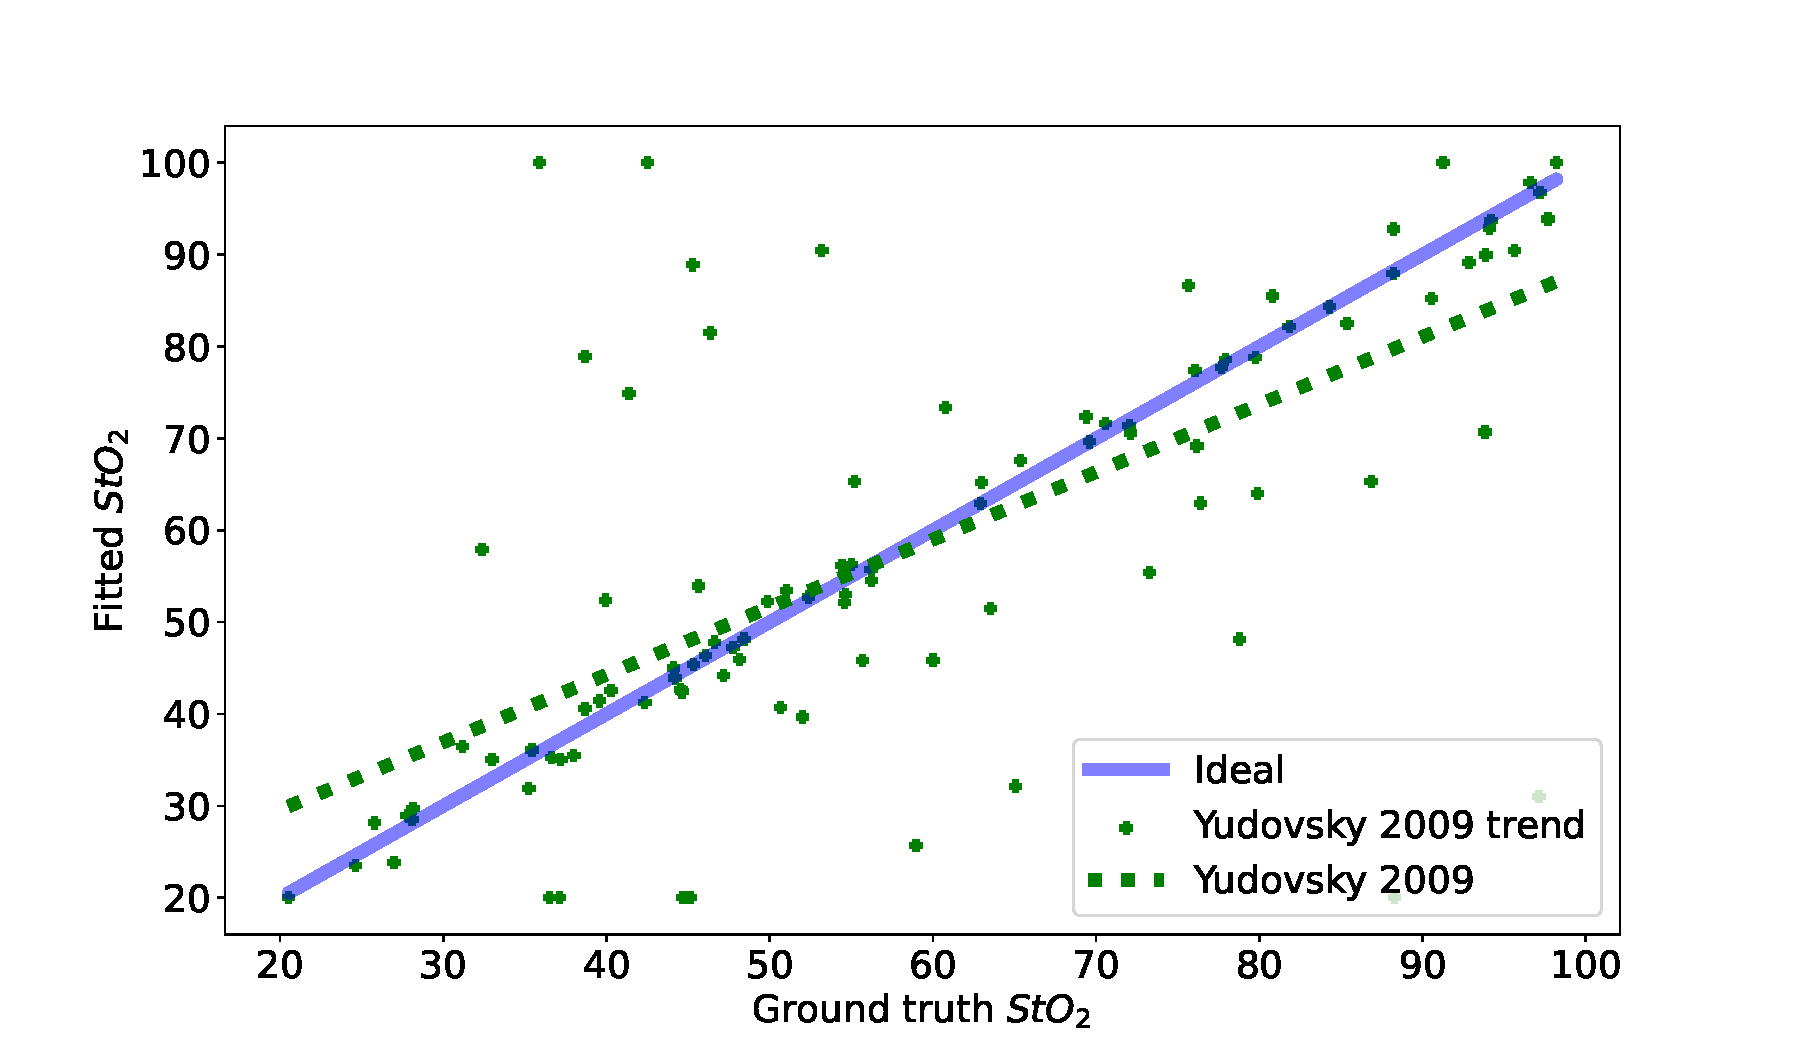
\includegraphics[width=\textwidth]{backwardsn0R2.pdf}
        \caption{}
        \label{fig:backwardsn0R2}
    \end{subfigure}
    \begin{subfigure}{0.49\textwidth}
        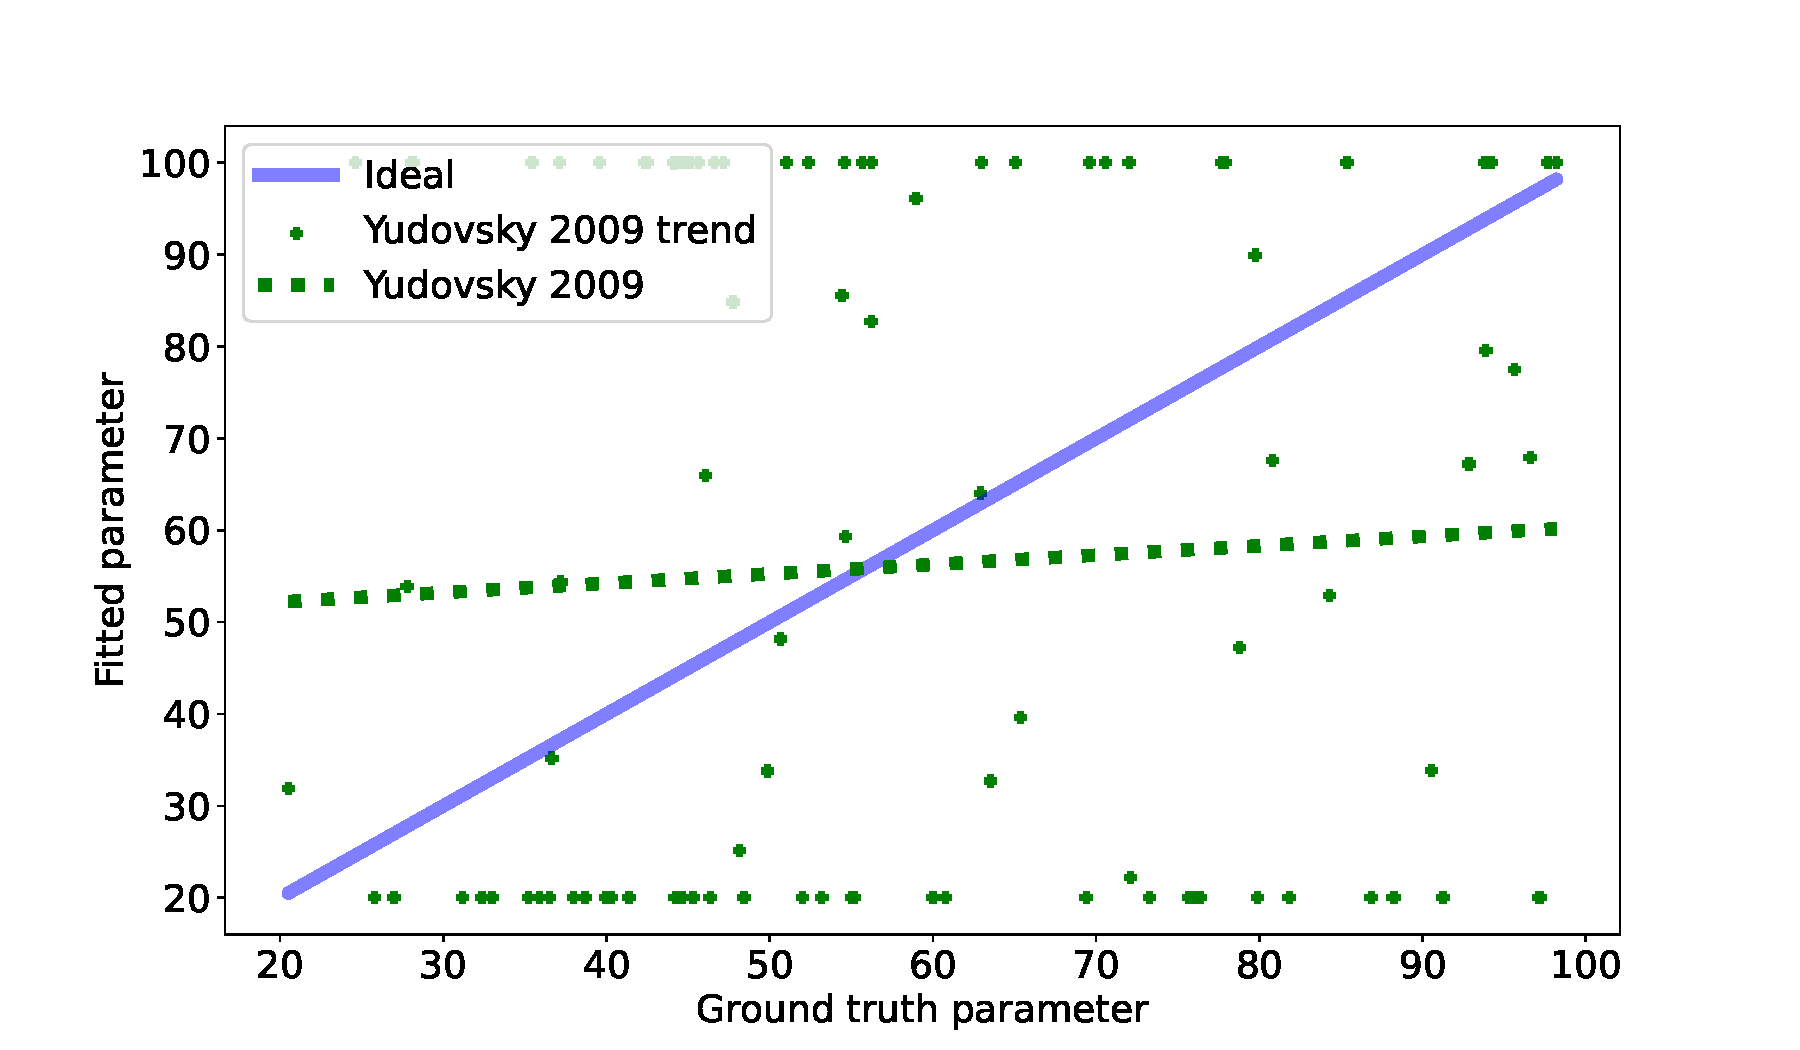
\includegraphics[width=\textwidth]{backwardsn0.01Q2.pdf}
        \caption{}
        \label{fig:backwardsn0.01Q2}
    \end{subfigure}
    \begin{subfigure}{0.49\textwidth}
        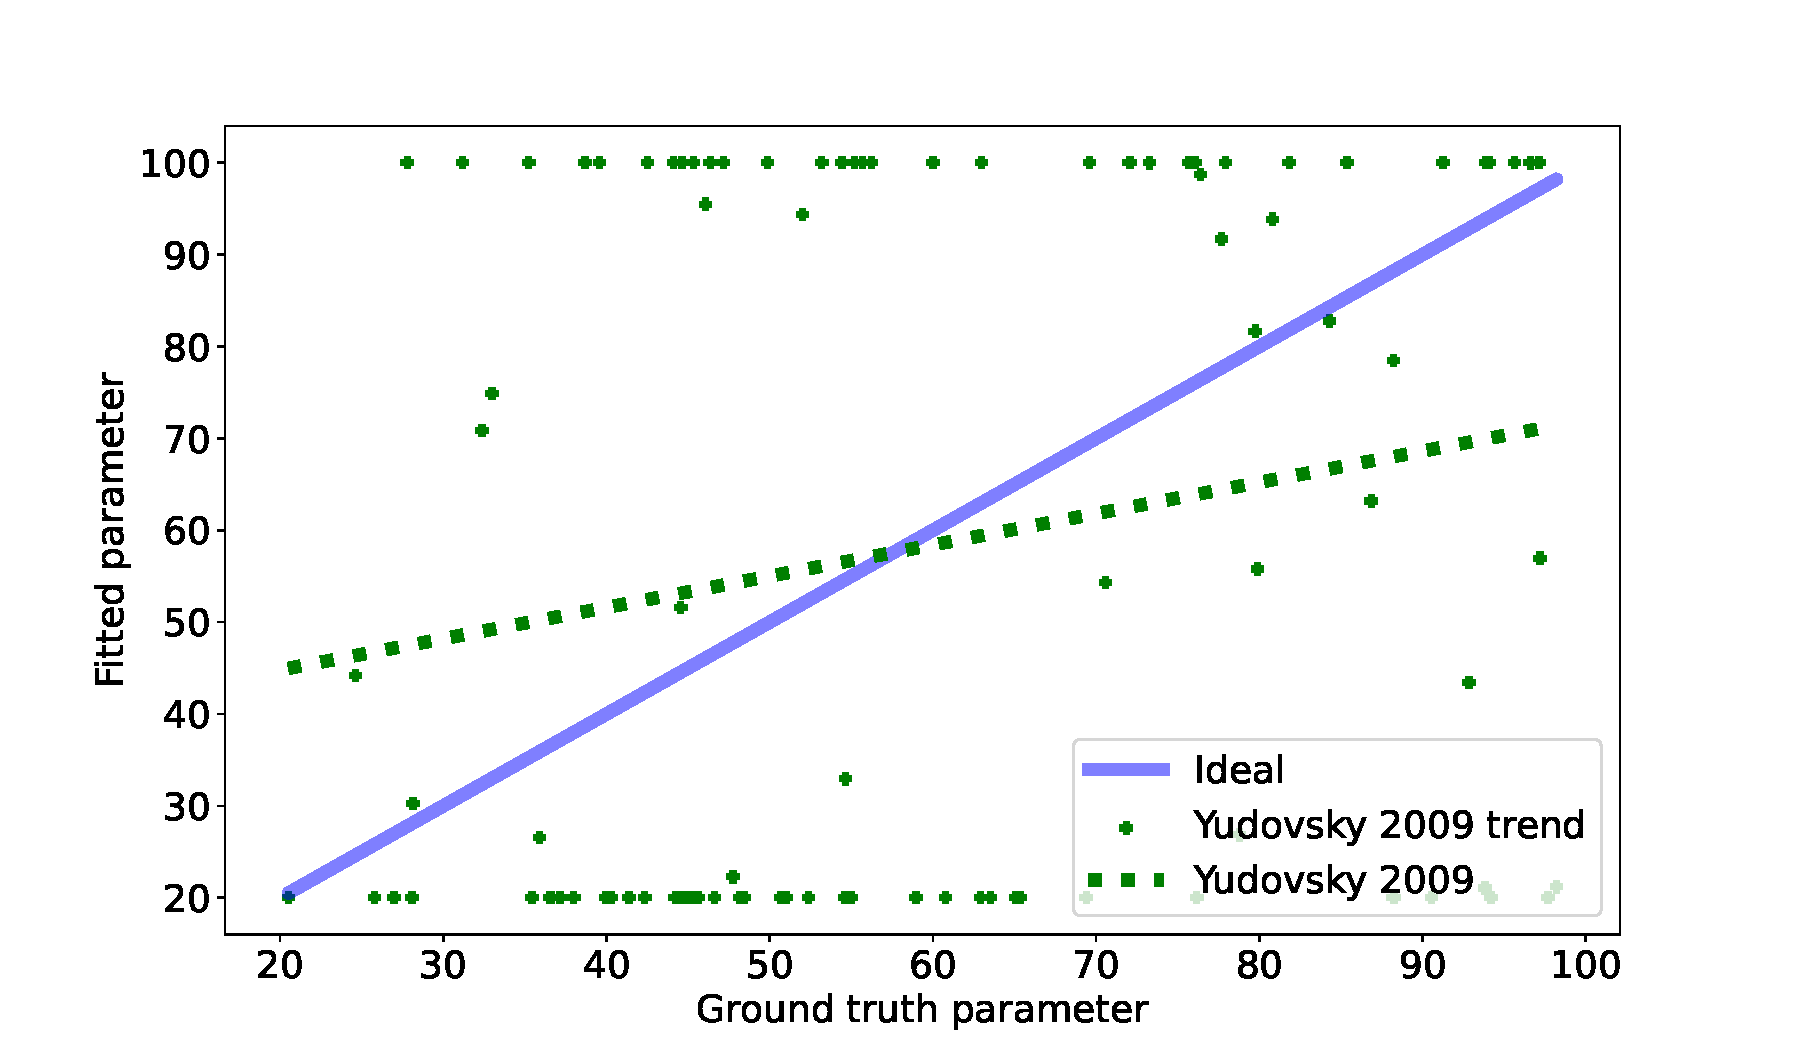
\includegraphics[width=\textwidth]{backwardsn0.01R2.pdf}
        \caption{}
        \label{fig:backwardsm0.01R2}
    \end{subfigure}
    \begin{subfigure}{0.49\textwidth}
        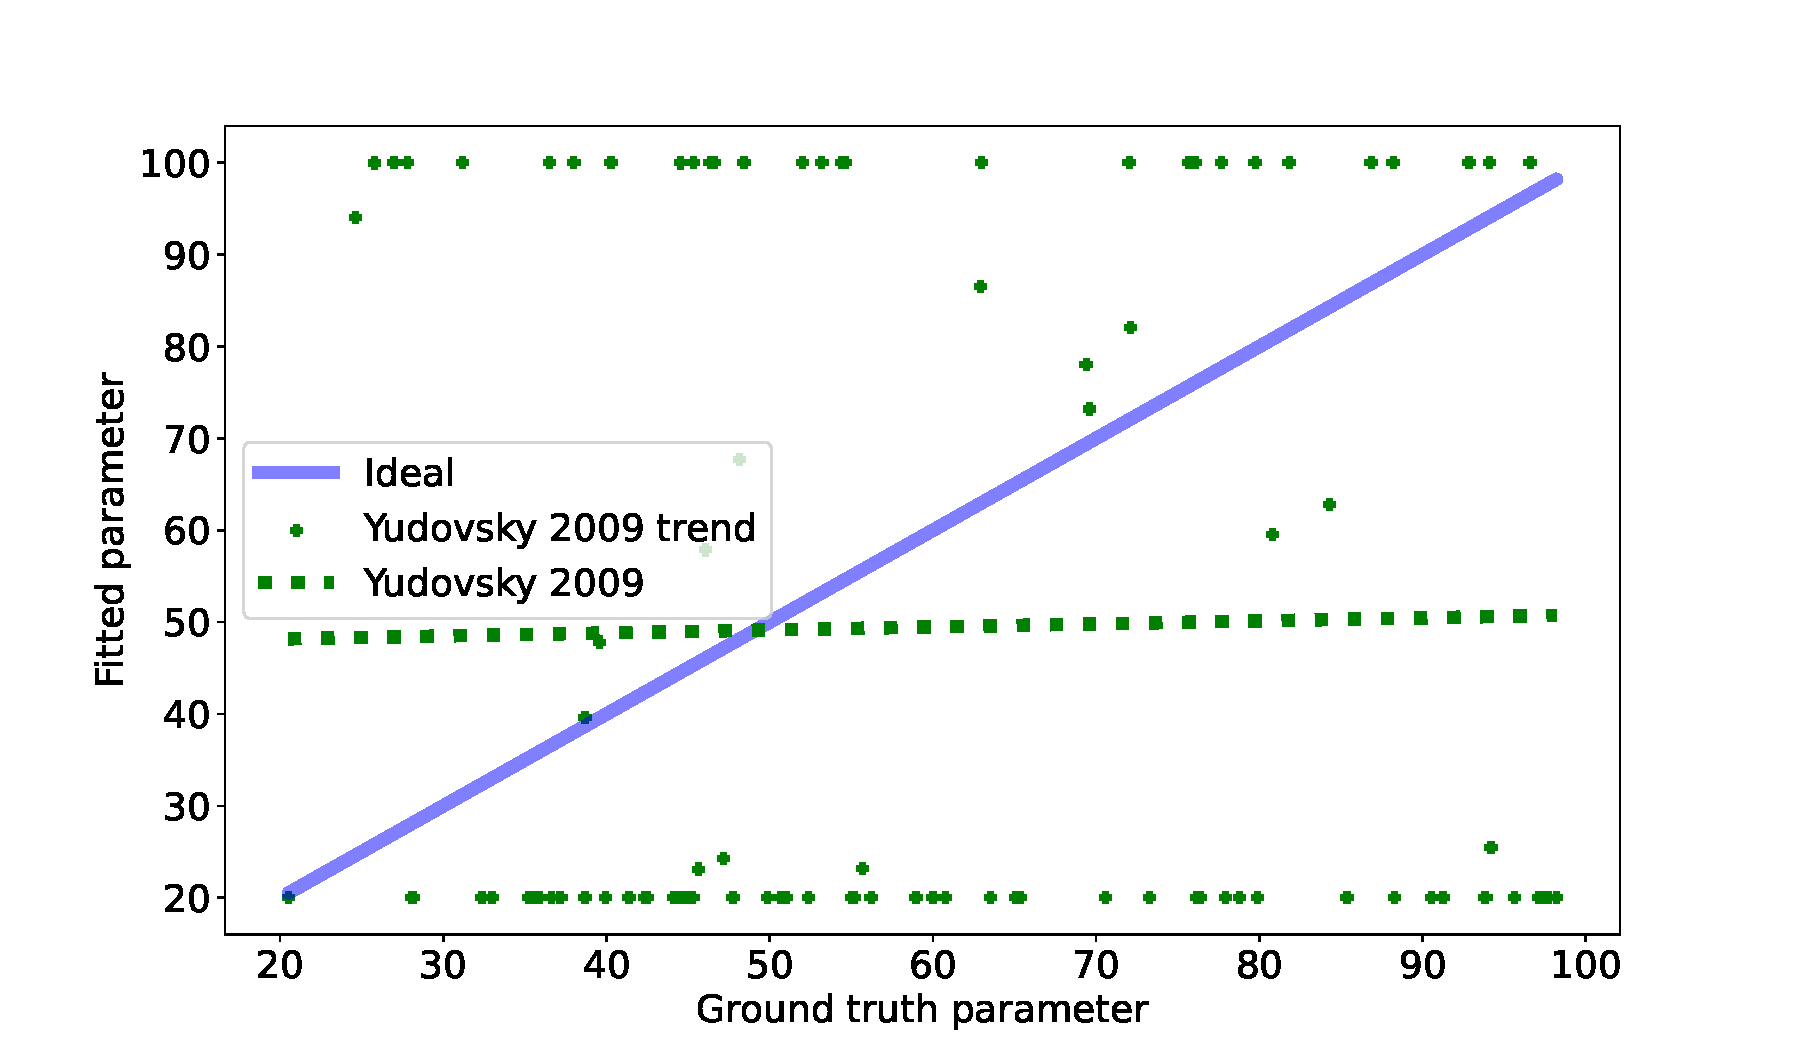
\includegraphics[width=\textwidth]{backwardsn0.03Q2.pdf}
        \caption{}
        \label{fig:backwardsn0.03Q2}
    \end{subfigure}
    \begin{subfigure}{0.49\textwidth}
        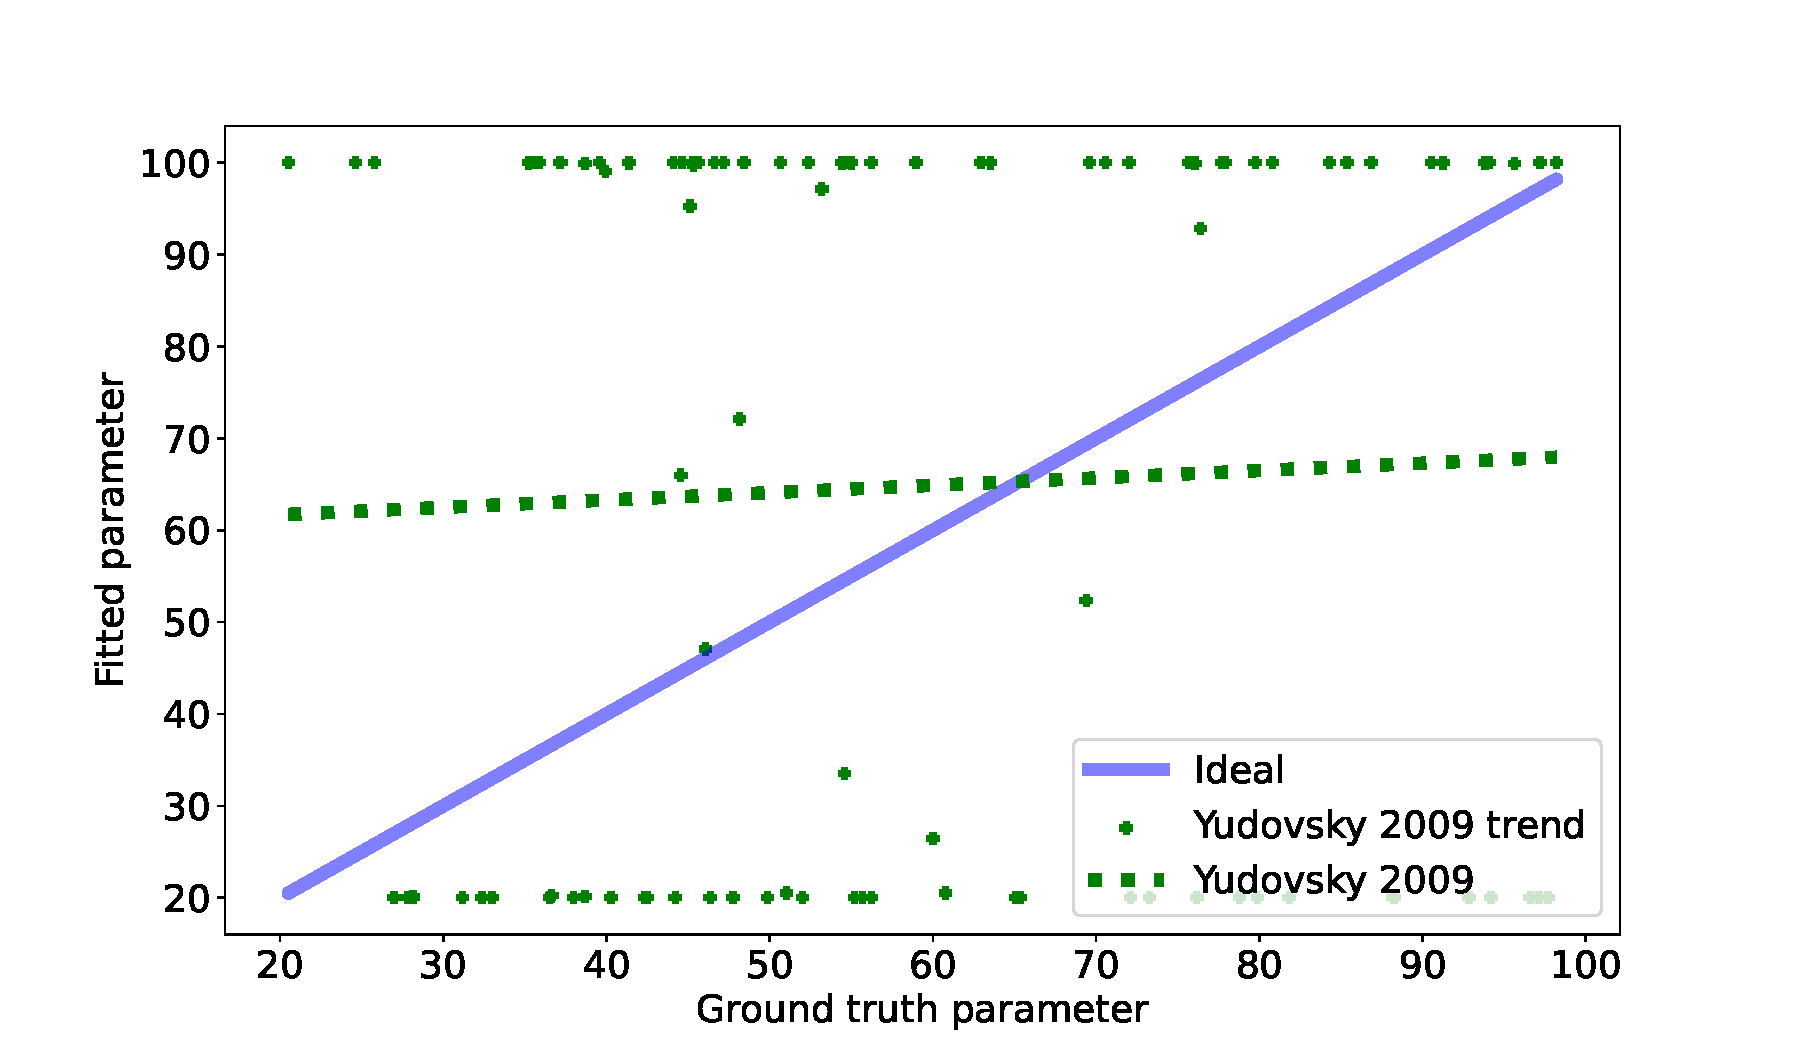
\includegraphics[width=\textwidth]{backwardsn0.03R2.pdf}
        \caption{}
        \label{fig:backwardsm0.03R2}
    \end{subfigure}
    \caption{An example of the quality of parameter recovery by fitting the double-layer inverse analytical model Yudovsky 2009 (\textcolor{MyGreen}{green $+$}) to the quantitative (left) or relative (right) simulated camera responses from the Monte Carlo simulations and their associated trend lines for a refractive index of 1.44 for $StO_2$. This is shown for data with either no added noise (top) or added noise with $\sigma = 0.01$ (middle) or $\sigma = 0.03$ (bottom).}
    \label{fig:backwardsHSIMC2}
\end{figure}

\subsection{Gelatin-based tissue phantoms}
To evaluate the quality of camera response simulation, the mean spectrum from the annotated region of each HSI image of a phantom is compared to the camera response simulation generated from the spectrophotometer diffuse reflectance measurement of these phantoms. This is also compared to the forwards models using ground truth parameters in Table \ref{tb:forwardsHSIphantoms} and an example seen in Figure \ref{fig:forwardsHSIphantoms}. 

\begin{table}[h!] %could remove noise levels here
    \centering
    \caption{Mean (standard deviation) $NRMSE$ (3.d.p.) between the simulated camera responses of each forwards spectrum from the Yudovsky 2009 single-layer model (Y1), the Jacques 1999 model (J), or using spectrophotometer measurements of each phantom (S) and each mean spectrum from an annotated HSI image of each phantom using the same ground truth variable parameters for quantitative and relative data. This is presented with the Pearson $r$ (bold if Pearson $p < 0.05$) for the linear regression between all forwards spectra against mean HSI phantom spectra for each analytical model or spectrophotometer measurements. All metrics are evaluated for the wavelength region of 450-600nm.}
    \begin{tabular}{|c|c|cc|}
        \hline
        Model & Quantitative (Q) & $NRMSE$ & $r$ \\
         & or Relative (R) &  & \\
        \hline
        \multirow{2}{*}{Y1} & Q & 0.138 (0.103) & \textbf{0.995} \\
        & R & 0.082 (0.048) & \textbf{0.994} \\
        \hline
        \multirow{2}{*}{J} & Q & 0.135 (0.108) & \textbf{0.995} \\
        & R & 0.088 (0.055) & \textbf{0.992} \\
        \hline
        \multirow{2}{*}{S} & Q & 0.201 (0.116) & \textbf{0.997} \\
         & R & 0.066 (0.044) & \textbf{0.994} \\
        \hline
    \end{tabular}
    \label{tb:forwardsHSIphantoms}
\end{table}

\begin{figure}[h!]
    \centering
    \begin{subfigure}{0.49\textwidth}
        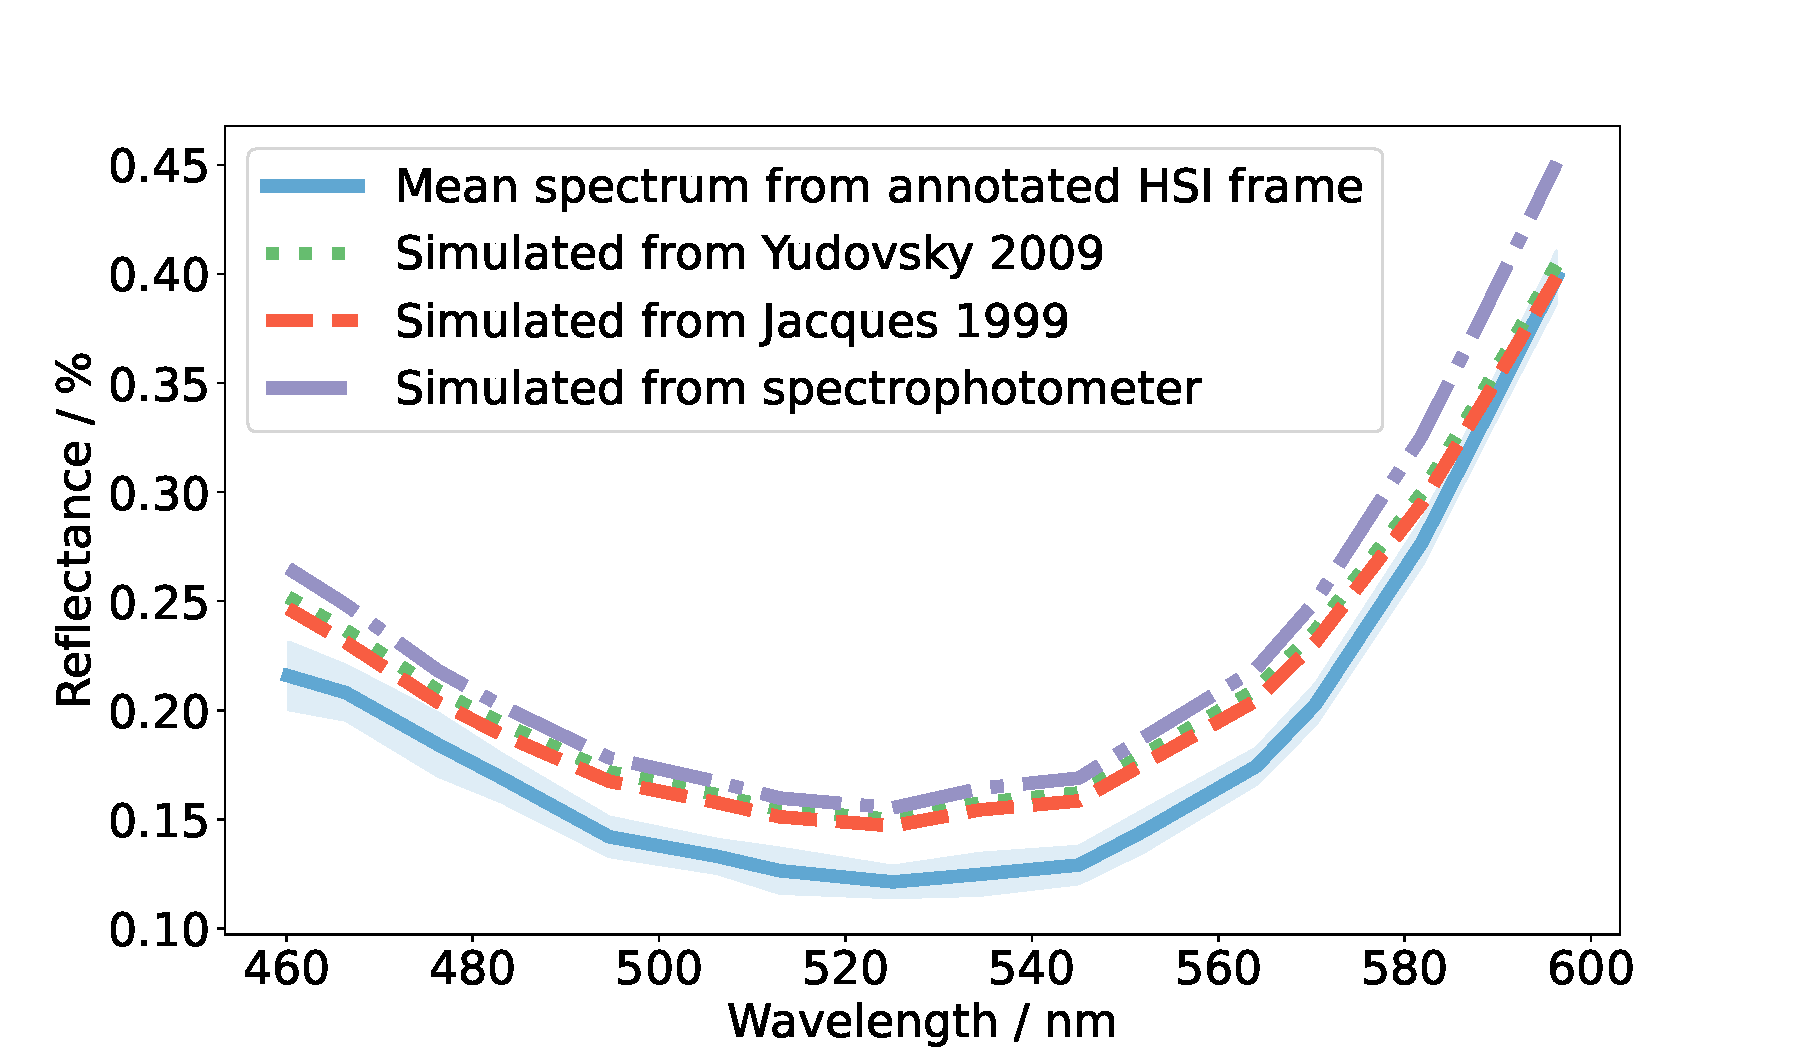
\includegraphics[width=\textwidth]{forwardsHSIphantomQ.pdf}
        \caption{}
        \label{fig:egforwardsHSIQ}
    \end{subfigure}
    \begin{subfigure}{0.49\textwidth}
        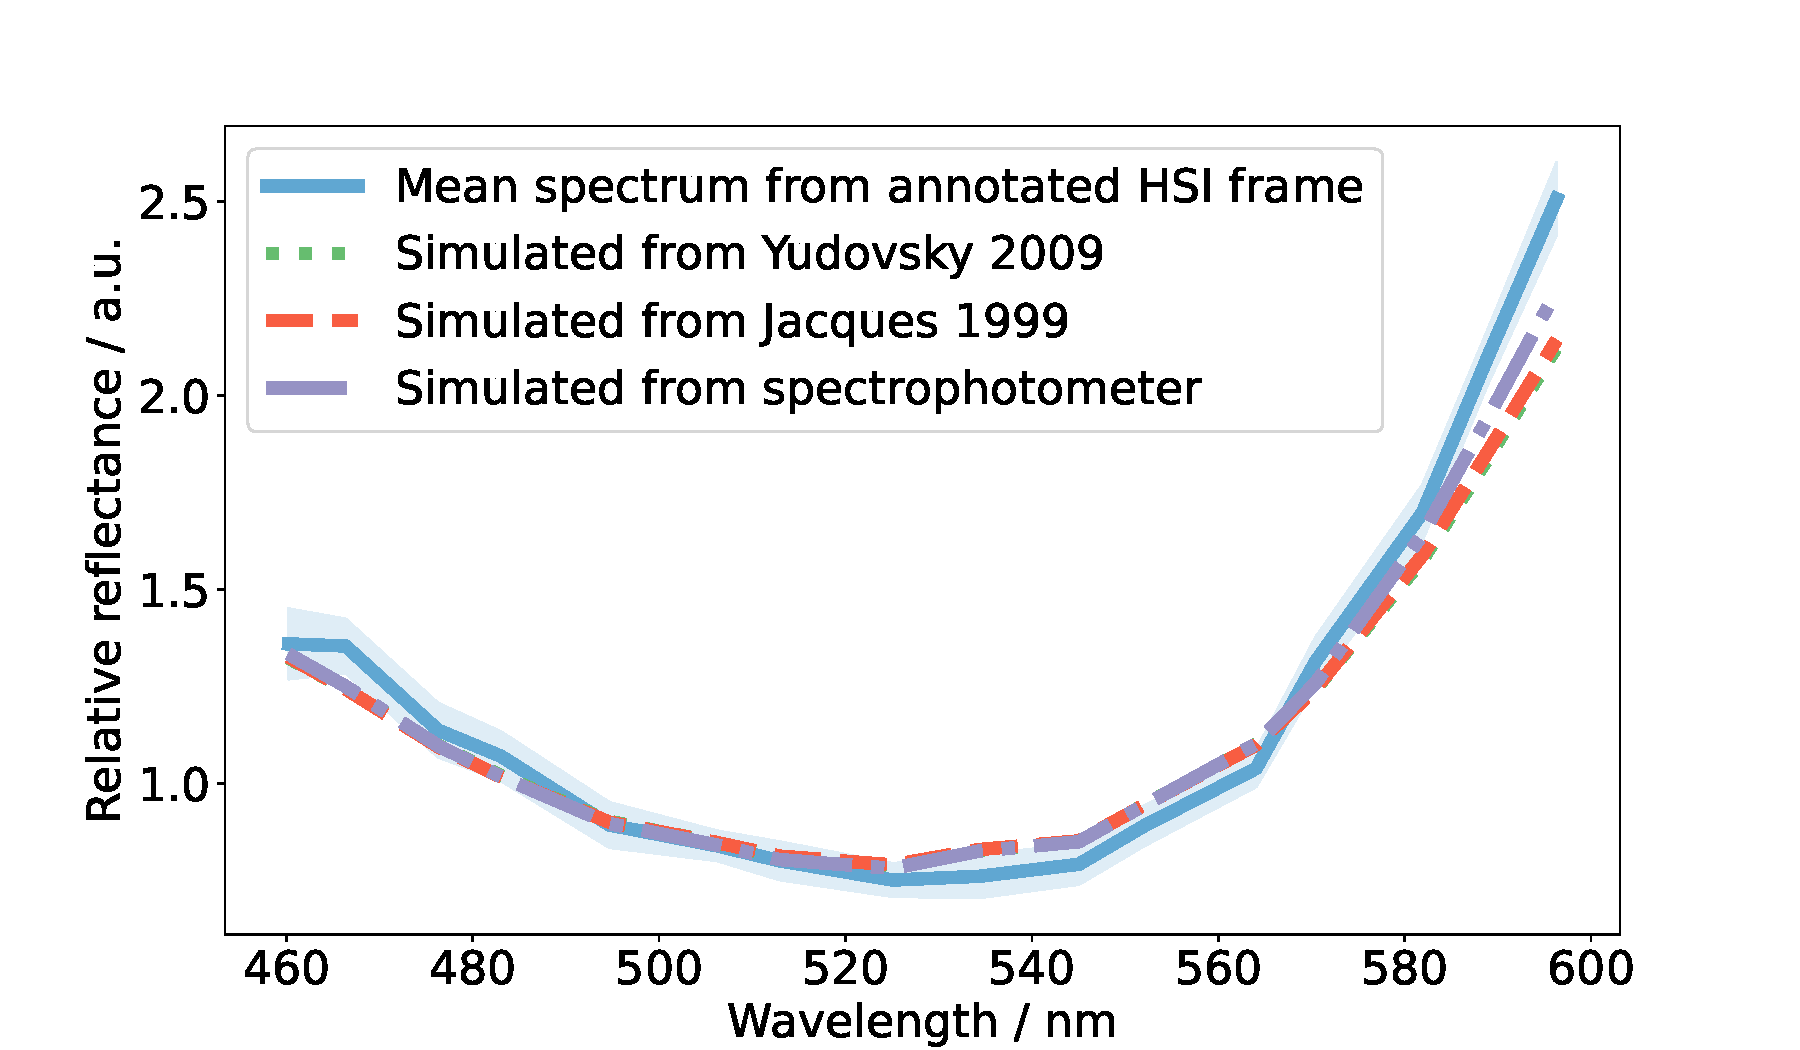
\includegraphics[width=\textwidth]{forwardsHSIphantomR.pdf}
        \caption{}
        \label{fig:egforwardsHSIR}
    \end{subfigure}
    \caption{Example of the simulated camera response spectra from each forward single-layer analytical model: Yudovsky 2009 (\textcolor{MyGreen}{green dotted}) and Jacques 1999 (\textcolor{MyOrange}{orange dashed}), using ground truth variables for a refractive index of 1.44 compared to that predicted using spectrophotometer measurements (\textcolor{purple}{purple dash-dotted} and the mean spectrum from an HSI image of the same phantom (\textcolor{MyBlue}{blue solid}) for quantitative (left) and relative (right) data.}
    \label{fig:forwardsHSIphantoms}
\end{figure}


\subsection{Neurosurgical HSI data}

\section{Discussion}